\documentclass[xcolor=svgnames,9pt,english,aspectratio=169,t]{beamer}
%\documentclass[xcolor=svgnames,9pt,english,handout,aspectratio=169,t]{beamer}
\newcommand{\handout}{0}

% =====================================================================
% POLI 450A (2026) --- shared TEMPLATE layer.
%
% Input from each lecture near the top of its file, BEFORE
% ../course_theme.tex (metropolis must be selected before the course
% palette overrides it):
%
%   \documentclass[xcolor=svgnames,9pt,english,aspectratio=169]{beamer}
%   \newcommand{\handout}{0}
%   % =====================================================================
% POLI 450A (2026) --- shared TEMPLATE layer.
%
% Input from each lecture near the top of its file, BEFORE
% ../course_theme.tex (metropolis must be selected before the course
% palette overrides it):
%
%   \documentclass[xcolor=svgnames,9pt,english,aspectratio=169]{beamer}
%   \newcommand{\handout}{0}
%   % =====================================================================
% POLI 450A (2026) --- shared TEMPLATE layer.
%
% Input from each lecture near the top of its file, BEFORE
% ../course_theme.tex (metropolis must be selected before the course
% palette overrides it):
%
%   \documentclass[xcolor=svgnames,9pt,english,aspectratio=169]{beamer}
%   \newcommand{\handout}{0}
%   \input{../course_preamble.tex}
%   \input{../course_theme.tex}
%   \graphicspath{{./}{./figs/}}
%   \title[Short title]{450A Political Methodology I}
%   \subtitle{Lecture N: ...}
%
% Modeled on the 2026 Northwestern workshop template
% (Teaching/PanelData/_latex/2026/202608_Northwestern/workshop_preamble.tex).
%
% SCOPE: theme, beamer layout, packages, the roadmap hooks, and --- unlike
% the Northwestern decks --- the notation macros. The 450A lectures
% grew from one common ancestor, so their macro blocks agree wherever they
% overlap; merging them is safe. Three points where they had drifted are
% resolved here, and each is flagged inline below.
% =====================================================================

\usetheme{metropolis}
\metroset{sectionpage=none, subsectionpage=none, numbering=none}
\setbeamertemplate{navigation symbols}{}

\setbeamersize{text margin left=5mm, text margin right=5mm}
\setbeamertemplate{itemize/enumerate body begin}{\leftmargini=1.5em\relax}
\setbeamertemplate{itemize/enumerate subbody begin}{\leftmarginii=1.5em\relax}
\setbeamertemplate{itemize/enumerate subsubbody begin}{\leftmarginiii=1.5em\relax}

% ----------------------------------------------------------- top alignment
% Every deck passes the t class option, so beamer applies the frame key
% below to every frame (explicit [plain,c] frames — title page, roadmaps —
% stay centered). Beamer's stock t key puts a rigid .2cm pad above the
% content; frames sized to this template's full-height ceilings then run
% Overfull \vbox by up to that pad. Same key as beamerbaseframe.sty, with
% one change: the pad may shrink to zero when the frame is full.
\makeatletter
\define@key{beamerframe}{t}[true]{% top
  \beamer@frametopskip=.2cm plus .5\paperheight minus .2cm\relax%
  \beamer@framebottomskip=0pt plus 1fill\relax%
  \beamer@frametopskipautobreak=\beamer@frametopskip\relax%
  \beamer@framebottomskipautobreak=\beamer@framebottomskip\relax%
}

% ------------------------------------------------- slide-top check (2026-10-11)
% A slide whose content is too tall for the frame is squeezed: the pad above
% shrinks and its content starts higher than on other slides, so a figure
% "wobbles" when the class steps from one slide to the next (Lecture 4-1,
% slides 1-2, 2026-10-11). The marker below records where each slide's
% content starts (a whatsit: it adds no space and moves nothing).
% `python3 ../check_slides.py lec<N>` then lists every slide that starts
% higher than the deck's normal position. That list must be empty.
% Recorded per slide: page, frame number, content-top y (sp), the room left
% below the title bar, and P for a plain frame (title page, roadmaps).
\providecommand\slidetop[5]{}
\AtBeginDocument{\immediate\write\@auxout{\string\providecommand\string\slidetop[5]{}}}
\def\beamer@markframetop{%
  \pdfsavepos
  \edef\beamer@marktmp{\noexpand\write\noexpand\@auxout{\string\slidetop
    {\noexpand\thepage}{\noexpand\insertframenumber}{\noexpand\the\noexpand\pdflastypos}%
    {\number\beamer@frametextheight}{\ifbeamer@plainframe P\else N\fi}}}%
  \beamer@marktmp}
\RequirePackage{etoolbox}
\patchcmd{\endbeamer@frameslide}
  {\vskip\beamer@frametopskip}
  {\vskip\beamer@frametopskip\beamer@markframetop}
  {}{\PackageWarning{course_preamble}{slide-top marker not installed}}
\makeatother

% ---------------------------------------------------------------- packages
\usepackage{xcolor}
\usepackage{colortbl}
\usepackage{amsmath}
\usepackage{amsfonts}
\usepackage{amssymb}
\usepackage{bm}
\usepackage{graphicx}
\usepackage{multirow}
\usepackage{fancyvrb}
\usepackage{listings}
\usepackage{tikz}
\usetikzlibrary{arrows.meta,positioning,decorations.pathreplacing}

% --------------------------------------------------------- figure fitting
% Default bounding box for every \includegraphics that does not override it.
% With keepaspectratio the image is scaled to fit *inside* width x height, so
% a figure can never run past the side margins or off the bottom of a slide.
% Options given at the call site override these on a per-key basis: e.g.
% [width=.6\linewidth] narrows the box but keeps the height ceiling.
% \figmaxheight is set at \begin{document}: beamer only computes the final
% \textheight once the head/foot templates are known. 0.80 is just under what a
% frame with a title and one line of text can hold (measured: 0.834\textheight);
% a frame that needs more room for text can lower it locally.
\newlength{\figmaxheight}
\AtBeginDocument{\setlength{\figmaxheight}{0.80\textheight}}
\setkeys{Gin}{width=\linewidth,height=\figmaxheight,keepaspectratio}

% -------------------------------------------------------- roadmap frames
% Identical in all lectures. A lecture that does not want the
% subsection roadmap clears it after the \input with \AtBeginSubsection[]{}.
% hideothersubsections is load-bearing, not cosmetic: lecture 4 had 13
% subsections before it was split into 4-1, 4-2 and 4-3 (2026-10-09), and a
% full contents list ran off the top and bottom of the slide. Hiding the other sections' subsections caps the list at 10 lines.
\subject{Talks}
% No back-to-back roadmaps (Yiqing, 2026-10-11): when a subsection starts right
% after its section's roadmap, with no content slide in between, its own
% roadmap would repeat the one just shown (5-1's handout showed "Two Cases"
% twice), so it is skipped. The section roadmap records the frame count; the
% subsection roadmap appears only if a content slide has come since.
\makeatletter
\def\course@secframe{-1}
\AtBeginSection[]
{
  \begin{frame}[plain,c]
    \frametitle{}
    \tableofcontents[currentsection,hideothersubsections]
    \addtocounter{framenumber}{-1}
  \end{frame}
  \xdef\course@secframe{\the\c@framenumber}
}
\AtBeginSubsection[]
{
  \ifnum\c@framenumber=\course@secframe\relax\else
  \begin{frame}[plain,c]
    \frametitle{}
    \tableofcontents[currentsection,currentsubsection,hideothersubsections]
    \addtocounter{framenumber}{-1}
  \end{frame}
  \fi
}
\makeatother

% ------------------------------------------------------ theorem environments
\newtheorem{assumption}{Assumption}
\newtheorem{iass}{Identification Assumption}
\newtheorem{ires}{Identification Result}
\newtheorem{estm}{Estimand}
\newtheorem{esti}{Estimator}
\newtheorem{question}{Question}
\newtheorem{answer}{Answer}
\newtheorem{proposition}{Proposition}

% =====================================================================
% Notation
% =====================================================================
\definecolor{dgreen}{rgb}{0,.6,0.8}

\renewcommand\r{\right}
\renewcommand\l{\left}
\newcommand{\bs}{\boldsymbol}
\newcommand{\mb}{\mathbf}
\newcommand{\real}{\mathbb{R}}
\newcommand{\cN}{\mathcal{N}}
\newcommand{\E}{\mathbb{E}}
\newcommand{\V}{\mathbb{V}}

% MERGE NOTE 1. Lecture 2-4 set \epsilon to \varepsilon; the other twelve
% left it at the upright default. Adopting \varepsilon course-wide so the
% error term looks the same in every lecture.
\renewcommand{\epsilon}{\varepsilon}

% MERGE NOTE 2. Lecture 2-4 wrote its vectors as \bm (bold italic); the other
% twelve use \mathbf (bold upright). \mathbf wins --- it is the convention in
% eleven of the thirteen decks and in the course's matrix lectures. Only
% \iid, \E, \cN and \Var from that block are actually used in 2-4's body.
\renewcommand{\u}{\ensuremath{\mb{u}}}
\renewcommand{\v}{\ensuremath{\mb{v}}}
\newcommand{\U}{\ensuremath{\mb{U}}}
\newcommand{\M}{\ensuremath{\mb{M}}}
\newcommand{\X}{\ensuremath{\mb{X}}}
\newcommand{\x}{\ensuremath{\mb{x}}}
\newcommand{\y}{\ensuremath{\mb{y}}}
\newcommand{\Z}{\ensuremath{\mb{Z}}}
\newcommand{\C}{\ensuremath{\mb{C}}}
\newcommand{\D}{\ensuremath{\mb{D}}}
\newcommand{\I}{\ensuremath{\mb{I}}}
\newcommand{\W}{\ensuremath{\mb{W}}}
\renewcommand{\a}{\ensuremath{\mb{a}}}
\renewcommand{\P}{\ensuremath{\mb{P}}}
\newcommand{\one}{\ensuremath{\mb{1}}}
\newcommand{\zero}{\ensuremath{\mb{0}}}

\renewcommand{\b}{\ensuremath{\bs{\beta}}}
\newcommand{\be}{\ensuremath{\bs{\beta}}}
\newcommand{\e}{\ensuremath{\bs{\epsilon}}}
\newcommand{\eps}{\ensuremath{\bs{\epsilon}}}
\newcommand{\eeta}{\ensuremath{\bs{\eta}}}
\newcommand{\bhat}{\ensuremath{\hat{\bs{\beta}}}}
\newcommand{\ehat}{\ensuremath{\hat{\e}}}
\newcommand{\Sig}{\ensuremath{\bs{\Sigma}}}
\newcommand{\SigInv}{\ensuremath{\bs{\Sigma^{-1}}}}

\newcommand{\XX}{\ensuremath{\X'\X}}
\newcommand{\XXinv}{\ensuremath{\left(\XX\right)^{-1}}}
\newcommand{\hatmat}{\ensuremath{\X \XXinv \X'}}
\newcommand{\hatsig}{\ensuremath{\hat{\sigma}^2}}
\newcommand{\sig}{\ensuremath{\sigma^2}}

\newcommand{\cA}{\mathcal{A}}
\newcommand{\cJ}{\mathcal{J}}
\newcommand{\cL}{\mathcal{L}}
\newcommand{\cLL}{\mathcal{LL}}
\newcommand{\cll}{\ell}
\newcommand{\cQ}{\mathcal{Q}}
\newcommand{\cP}{\mathcal{P}}

% MERGE NOTE 3. \var / \Var and \cov / \Cov were spelled with \text in some
% lectures and \mbox in others. Same output; \text kept.
\newcommand{\var}{\text{Var}}
\newcommand{\Var}{\text{Var}}
\newcommand{\cov}{\text{Cov}}
\newcommand{\Cov}{\text{Cov}}
\newcommand{\cor}{\text{Cor}}
\newcommand{\tr}{\text{tr}}
\newcommand{\avepop}{\frac{1}{n}\sum_{i=1}^n}

\DeclareMathOperator*\plim{plim}
\DeclareMathOperator\rank{rank}
\DeclareMathOperator*\argmax{argmax}
\DeclareMathOperator*\argmin{argmin}
\DeclareMathOperator{\sgn}{sgn}
\newcommand{\diag}{\mathop{\mathrm{diag}}}

\newcommand\ud{\mathrm{d}}
\newcommand\dist{\buildrel\rm d\over\sim}
\newcommand\ind{\stackrel{\rm indep.}{\sim}}
\newcommand\iid{\stackrel{\rm i.i.d.}{\sim}}
\newcommand\logit{{\rm logit}}

\newcommand\indep{\protect\mathpalette{\protect\independenT}{\perp}}
\def\independenT#1#2{\mathrel{\rlap{$#1#2$}\mkern2mu{#1#2}}}

% ------------------------------------------------------------- text helpers
\newcommand{\bi}{\begin{itemize}}
\newcommand{\ei}{\end{itemize}}
\newcommand{\noi}{\noindent}
\newcommand{\red}{\textcolor{Cardinal}}
\newcommand{\blue}{\textcolor{CourseBlue}}
\newcommand{\gray}{\textcolor{gray}}
\newcommand\spacingset[1]{\renewcommand{\baselinestretch}{#1}\small\normalsize}

\hyphenation{tyamamot}


% ------------------------------------------------ figure-position check (2026-10-11)
% Records where every \includegraphics lands and its size (a whatsit; it moves
% nothing). check_slides.py flags two consecutive slides that show a figure of
% the same size in different places: the class sees it jump (Lecture 3, slides
% 18 to 19: one frame had \vspace{.3cm} above the figure, the next did not),
% and two consecutive slides that show the same file at different sizes or
% places (Lecture 6-3, slides 10 to 11, the ballot image). The file name is the
% seventh field.
\makeatletter
\providecommand\figpos[7]{}
\AtBeginDocument{\immediate\write\@auxout{\string\providecommand\string\figpos[7]{}}}
\newbox\course@figbox
\let\course@origGinclude\Ginclude@graphics
\def\Ginclude@graphics#1{%
  \setbox\course@figbox\hbox{\course@origGinclude{#1}}%
  \pdfsavepos
  \edef\course@figtmp{\noexpand\write\noexpand\@auxout{\string\figpos
    {\noexpand\thepage}{\noexpand\insertframenumber}%
    {\noexpand\the\noexpand\pdflastxpos}{\noexpand\the\noexpand\pdflastypos}%
    {\number\wd\course@figbox}{\number\ht\course@figbox}{\detokenize{#1}}}}%
  \course@figtmp
  \box\course@figbox}
\makeatother

%   % =====================================================================
% POLI 450A (2026) --- shared visual system.
% Input from each lecture AFTER ../course_preamble.tex.
%
% Same shape as the 2026 Northwestern workshop theme
% (Teaching/PanelData/_latex/2026/202608_Northwestern/workshop_theme.tex),
% with the workshop's purple swapped for the course's cardinal. Kept
% deliberately light so the lecture sources stay easy to edit.
%
% To retune the course to Stanford's official cardinal, change the one
% Cardinal line below to HTML 8C1515.
% =====================================================================
\definecolor{Cardinal}{HTML}{A8003B}     % primary: titles, structure, alerts
\definecolor{CourseInk}{HTML}{252A34}    % body text
\definecolor{CourseBlue}{HTML}{2F6B9A}   % secondary accent
\definecolor{CourseMist}{HTML}{F8F1F4}   % block backgrounds

\setbeamercolor{normal text}{fg=CourseInk,bg=white}
\setbeamercolor{structure}{fg=Cardinal}
\setbeamercolor{alerted text}{fg=Cardinal}
\setbeamercolor{frametitle}{fg=white,bg=Cardinal}
\setbeamercolor{title}{fg=Cardinal}
\setbeamercolor{subtitle}{fg=CourseInk}
\setbeamercolor{block title}{fg=white,bg=Cardinal}
\setbeamercolor{block body}{fg=CourseInk,bg=CourseMist}
\setbeamercolor{section in toc}{fg=Cardinal}
\setbeamercolor{subsection in toc}{fg=CourseInk}
\setbeamercolor{itemize item}{fg=Cardinal}
\setbeamercolor{itemize subitem}{fg=Cardinal}
\setbeamercolor{enumerate item}{fg=Cardinal}

\setbeamerfont{title}{series=\bfseries,size=\Large}
\setbeamerfont{frametitle}{series=\bfseries,size=\large}
\setbeamerfont{block title}{series=\bfseries}
\setbeamertemplate{navigation symbols}{}
\setbeamertemplate{items}[circle]
\setbeamertemplate{blocks}[rounded][shadow=false]
\setbeamertemplate{frametitle continuation}{}
\setbeamertemplate{footline}{%
  \leavevmode\hbox{%
  \begin{beamercolorbox}[wd=.88\paperwidth,ht=2.6ex,dp=1.2ex,leftskip=1.2em]{author in head/foot}%
  \usebeamerfont{author in head/foot}\insertshorttitle
  \end{beamercolorbox}%
  \begin{beamercolorbox}[wd=.12\paperwidth,ht=2.6ex,dp=1.2ex,center]{date in head/foot}%
  \insertframenumber
  \end{beamercolorbox}}}

\newcommand{\slidesource}[1]{\vfill{\scriptsize\color{gray}Source: #1}}
\newcommand{\keyquestion}[1]{\begin{block}{Question}#1\end{block}}

%   \graphicspath{{./}{./figs/}}
%   \title[Short title]{450A Political Methodology I}
%   \subtitle{Lecture N: ...}
%
% Modeled on the 2026 Northwestern workshop template
% (Teaching/PanelData/_latex/2026/202608_Northwestern/workshop_preamble.tex).
%
% SCOPE: theme, beamer layout, packages, the roadmap hooks, and --- unlike
% the Northwestern decks --- the notation macros. The 450A lectures
% grew from one common ancestor, so their macro blocks agree wherever they
% overlap; merging them is safe. Three points where they had drifted are
% resolved here, and each is flagged inline below.
% =====================================================================

\usetheme{metropolis}
\metroset{sectionpage=none, subsectionpage=none, numbering=none}
\setbeamertemplate{navigation symbols}{}

\setbeamersize{text margin left=5mm, text margin right=5mm}
\setbeamertemplate{itemize/enumerate body begin}{\leftmargini=1.5em\relax}
\setbeamertemplate{itemize/enumerate subbody begin}{\leftmarginii=1.5em\relax}
\setbeamertemplate{itemize/enumerate subsubbody begin}{\leftmarginiii=1.5em\relax}

% ----------------------------------------------------------- top alignment
% Every deck passes the t class option, so beamer applies the frame key
% below to every frame (explicit [plain,c] frames — title page, roadmaps —
% stay centered). Beamer's stock t key puts a rigid .2cm pad above the
% content; frames sized to this template's full-height ceilings then run
% Overfull \vbox by up to that pad. Same key as beamerbaseframe.sty, with
% one change: the pad may shrink to zero when the frame is full.
\makeatletter
\define@key{beamerframe}{t}[true]{% top
  \beamer@frametopskip=.2cm plus .5\paperheight minus .2cm\relax%
  \beamer@framebottomskip=0pt plus 1fill\relax%
  \beamer@frametopskipautobreak=\beamer@frametopskip\relax%
  \beamer@framebottomskipautobreak=\beamer@framebottomskip\relax%
}

% ------------------------------------------------- slide-top check (2026-10-11)
% A slide whose content is too tall for the frame is squeezed: the pad above
% shrinks and its content starts higher than on other slides, so a figure
% "wobbles" when the class steps from one slide to the next (Lecture 4-1,
% slides 1-2, 2026-10-11). The marker below records where each slide's
% content starts (a whatsit: it adds no space and moves nothing).
% `python3 ../check_slides.py lec<N>` then lists every slide that starts
% higher than the deck's normal position. That list must be empty.
% Recorded per slide: page, frame number, content-top y (sp), the room left
% below the title bar, and P for a plain frame (title page, roadmaps).
\providecommand\slidetop[5]{}
\AtBeginDocument{\immediate\write\@auxout{\string\providecommand\string\slidetop[5]{}}}
\def\beamer@markframetop{%
  \pdfsavepos
  \edef\beamer@marktmp{\noexpand\write\noexpand\@auxout{\string\slidetop
    {\noexpand\thepage}{\noexpand\insertframenumber}{\noexpand\the\noexpand\pdflastypos}%
    {\number\beamer@frametextheight}{\ifbeamer@plainframe P\else N\fi}}}%
  \beamer@marktmp}
\RequirePackage{etoolbox}
\patchcmd{\endbeamer@frameslide}
  {\vskip\beamer@frametopskip}
  {\vskip\beamer@frametopskip\beamer@markframetop}
  {}{\PackageWarning{course_preamble}{slide-top marker not installed}}
\makeatother

% ---------------------------------------------------------------- packages
\usepackage{xcolor}
\usepackage{colortbl}
\usepackage{amsmath}
\usepackage{amsfonts}
\usepackage{amssymb}
\usepackage{bm}
\usepackage{graphicx}
\usepackage{multirow}
\usepackage{fancyvrb}
\usepackage{listings}
\usepackage{tikz}
\usetikzlibrary{arrows.meta,positioning,decorations.pathreplacing}

% --------------------------------------------------------- figure fitting
% Default bounding box for every \includegraphics that does not override it.
% With keepaspectratio the image is scaled to fit *inside* width x height, so
% a figure can never run past the side margins or off the bottom of a slide.
% Options given at the call site override these on a per-key basis: e.g.
% [width=.6\linewidth] narrows the box but keeps the height ceiling.
% \figmaxheight is set at \begin{document}: beamer only computes the final
% \textheight once the head/foot templates are known. 0.80 is just under what a
% frame with a title and one line of text can hold (measured: 0.834\textheight);
% a frame that needs more room for text can lower it locally.
\newlength{\figmaxheight}
\AtBeginDocument{\setlength{\figmaxheight}{0.80\textheight}}
\setkeys{Gin}{width=\linewidth,height=\figmaxheight,keepaspectratio}

% -------------------------------------------------------- roadmap frames
% Identical in all lectures. A lecture that does not want the
% subsection roadmap clears it after the \input with \AtBeginSubsection[]{}.
% hideothersubsections is load-bearing, not cosmetic: lecture 4 had 13
% subsections before it was split into 4-1, 4-2 and 4-3 (2026-10-09), and a
% full contents list ran off the top and bottom of the slide. Hiding the other sections' subsections caps the list at 10 lines.
\subject{Talks}
% No back-to-back roadmaps (Yiqing, 2026-10-11): when a subsection starts right
% after its section's roadmap, with no content slide in between, its own
% roadmap would repeat the one just shown (5-1's handout showed "Two Cases"
% twice), so it is skipped. The section roadmap records the frame count; the
% subsection roadmap appears only if a content slide has come since.
\makeatletter
\def\course@secframe{-1}
\AtBeginSection[]
{
  \begin{frame}[plain,c]
    \frametitle{}
    \tableofcontents[currentsection,hideothersubsections]
    \addtocounter{framenumber}{-1}
  \end{frame}
  \xdef\course@secframe{\the\c@framenumber}
}
\AtBeginSubsection[]
{
  \ifnum\c@framenumber=\course@secframe\relax\else
  \begin{frame}[plain,c]
    \frametitle{}
    \tableofcontents[currentsection,currentsubsection,hideothersubsections]
    \addtocounter{framenumber}{-1}
  \end{frame}
  \fi
}
\makeatother

% ------------------------------------------------------ theorem environments
\newtheorem{assumption}{Assumption}
\newtheorem{iass}{Identification Assumption}
\newtheorem{ires}{Identification Result}
\newtheorem{estm}{Estimand}
\newtheorem{esti}{Estimator}
\newtheorem{question}{Question}
\newtheorem{answer}{Answer}
\newtheorem{proposition}{Proposition}

% =====================================================================
% Notation
% =====================================================================
\definecolor{dgreen}{rgb}{0,.6,0.8}

\renewcommand\r{\right}
\renewcommand\l{\left}
\newcommand{\bs}{\boldsymbol}
\newcommand{\mb}{\mathbf}
\newcommand{\real}{\mathbb{R}}
\newcommand{\cN}{\mathcal{N}}
\newcommand{\E}{\mathbb{E}}
\newcommand{\V}{\mathbb{V}}

% MERGE NOTE 1. Lecture 2-4 set \epsilon to \varepsilon; the other twelve
% left it at the upright default. Adopting \varepsilon course-wide so the
% error term looks the same in every lecture.
\renewcommand{\epsilon}{\varepsilon}

% MERGE NOTE 2. Lecture 2-4 wrote its vectors as \bm (bold italic); the other
% twelve use \mathbf (bold upright). \mathbf wins --- it is the convention in
% eleven of the thirteen decks and in the course's matrix lectures. Only
% \iid, \E, \cN and \Var from that block are actually used in 2-4's body.
\renewcommand{\u}{\ensuremath{\mb{u}}}
\renewcommand{\v}{\ensuremath{\mb{v}}}
\newcommand{\U}{\ensuremath{\mb{U}}}
\newcommand{\M}{\ensuremath{\mb{M}}}
\newcommand{\X}{\ensuremath{\mb{X}}}
\newcommand{\x}{\ensuremath{\mb{x}}}
\newcommand{\y}{\ensuremath{\mb{y}}}
\newcommand{\Z}{\ensuremath{\mb{Z}}}
\newcommand{\C}{\ensuremath{\mb{C}}}
\newcommand{\D}{\ensuremath{\mb{D}}}
\newcommand{\I}{\ensuremath{\mb{I}}}
\newcommand{\W}{\ensuremath{\mb{W}}}
\renewcommand{\a}{\ensuremath{\mb{a}}}
\renewcommand{\P}{\ensuremath{\mb{P}}}
\newcommand{\one}{\ensuremath{\mb{1}}}
\newcommand{\zero}{\ensuremath{\mb{0}}}

\renewcommand{\b}{\ensuremath{\bs{\beta}}}
\newcommand{\be}{\ensuremath{\bs{\beta}}}
\newcommand{\e}{\ensuremath{\bs{\epsilon}}}
\newcommand{\eps}{\ensuremath{\bs{\epsilon}}}
\newcommand{\eeta}{\ensuremath{\bs{\eta}}}
\newcommand{\bhat}{\ensuremath{\hat{\bs{\beta}}}}
\newcommand{\ehat}{\ensuremath{\hat{\e}}}
\newcommand{\Sig}{\ensuremath{\bs{\Sigma}}}
\newcommand{\SigInv}{\ensuremath{\bs{\Sigma^{-1}}}}

\newcommand{\XX}{\ensuremath{\X'\X}}
\newcommand{\XXinv}{\ensuremath{\left(\XX\right)^{-1}}}
\newcommand{\hatmat}{\ensuremath{\X \XXinv \X'}}
\newcommand{\hatsig}{\ensuremath{\hat{\sigma}^2}}
\newcommand{\sig}{\ensuremath{\sigma^2}}

\newcommand{\cA}{\mathcal{A}}
\newcommand{\cJ}{\mathcal{J}}
\newcommand{\cL}{\mathcal{L}}
\newcommand{\cLL}{\mathcal{LL}}
\newcommand{\cll}{\ell}
\newcommand{\cQ}{\mathcal{Q}}
\newcommand{\cP}{\mathcal{P}}

% MERGE NOTE 3. \var / \Var and \cov / \Cov were spelled with \text in some
% lectures and \mbox in others. Same output; \text kept.
\newcommand{\var}{\text{Var}}
\newcommand{\Var}{\text{Var}}
\newcommand{\cov}{\text{Cov}}
\newcommand{\Cov}{\text{Cov}}
\newcommand{\cor}{\text{Cor}}
\newcommand{\tr}{\text{tr}}
\newcommand{\avepop}{\frac{1}{n}\sum_{i=1}^n}

\DeclareMathOperator*\plim{plim}
\DeclareMathOperator\rank{rank}
\DeclareMathOperator*\argmax{argmax}
\DeclareMathOperator*\argmin{argmin}
\DeclareMathOperator{\sgn}{sgn}
\newcommand{\diag}{\mathop{\mathrm{diag}}}

\newcommand\ud{\mathrm{d}}
\newcommand\dist{\buildrel\rm d\over\sim}
\newcommand\ind{\stackrel{\rm indep.}{\sim}}
\newcommand\iid{\stackrel{\rm i.i.d.}{\sim}}
\newcommand\logit{{\rm logit}}

\newcommand\indep{\protect\mathpalette{\protect\independenT}{\perp}}
\def\independenT#1#2{\mathrel{\rlap{$#1#2$}\mkern2mu{#1#2}}}

% ------------------------------------------------------------- text helpers
\newcommand{\bi}{\begin{itemize}}
\newcommand{\ei}{\end{itemize}}
\newcommand{\noi}{\noindent}
\newcommand{\red}{\textcolor{Cardinal}}
\newcommand{\blue}{\textcolor{CourseBlue}}
\newcommand{\gray}{\textcolor{gray}}
\newcommand\spacingset[1]{\renewcommand{\baselinestretch}{#1}\small\normalsize}

\hyphenation{tyamamot}


% ------------------------------------------------ figure-position check (2026-10-11)
% Records where every \includegraphics lands and its size (a whatsit; it moves
% nothing). check_slides.py flags two consecutive slides that show a figure of
% the same size in different places: the class sees it jump (Lecture 3, slides
% 18 to 19: one frame had \vspace{.3cm} above the figure, the next did not),
% and two consecutive slides that show the same file at different sizes or
% places (Lecture 6-3, slides 10 to 11, the ballot image). The file name is the
% seventh field.
\makeatletter
\providecommand\figpos[7]{}
\AtBeginDocument{\immediate\write\@auxout{\string\providecommand\string\figpos[7]{}}}
\newbox\course@figbox
\let\course@origGinclude\Ginclude@graphics
\def\Ginclude@graphics#1{%
  \setbox\course@figbox\hbox{\course@origGinclude{#1}}%
  \pdfsavepos
  \edef\course@figtmp{\noexpand\write\noexpand\@auxout{\string\figpos
    {\noexpand\thepage}{\noexpand\insertframenumber}%
    {\noexpand\the\noexpand\pdflastxpos}{\noexpand\the\noexpand\pdflastypos}%
    {\number\wd\course@figbox}{\number\ht\course@figbox}{\detokenize{#1}}}}%
  \course@figtmp
  \box\course@figbox}
\makeatother

%   % =====================================================================
% POLI 450A (2026) --- shared visual system.
% Input from each lecture AFTER ../course_preamble.tex.
%
% Same shape as the 2026 Northwestern workshop theme
% (Teaching/PanelData/_latex/2026/202608_Northwestern/workshop_theme.tex),
% with the workshop's purple swapped for the course's cardinal. Kept
% deliberately light so the lecture sources stay easy to edit.
%
% To retune the course to Stanford's official cardinal, change the one
% Cardinal line below to HTML 8C1515.
% =====================================================================
\definecolor{Cardinal}{HTML}{A8003B}     % primary: titles, structure, alerts
\definecolor{CourseInk}{HTML}{252A34}    % body text
\definecolor{CourseBlue}{HTML}{2F6B9A}   % secondary accent
\definecolor{CourseMist}{HTML}{F8F1F4}   % block backgrounds

\setbeamercolor{normal text}{fg=CourseInk,bg=white}
\setbeamercolor{structure}{fg=Cardinal}
\setbeamercolor{alerted text}{fg=Cardinal}
\setbeamercolor{frametitle}{fg=white,bg=Cardinal}
\setbeamercolor{title}{fg=Cardinal}
\setbeamercolor{subtitle}{fg=CourseInk}
\setbeamercolor{block title}{fg=white,bg=Cardinal}
\setbeamercolor{block body}{fg=CourseInk,bg=CourseMist}
\setbeamercolor{section in toc}{fg=Cardinal}
\setbeamercolor{subsection in toc}{fg=CourseInk}
\setbeamercolor{itemize item}{fg=Cardinal}
\setbeamercolor{itemize subitem}{fg=Cardinal}
\setbeamercolor{enumerate item}{fg=Cardinal}

\setbeamerfont{title}{series=\bfseries,size=\Large}
\setbeamerfont{frametitle}{series=\bfseries,size=\large}
\setbeamerfont{block title}{series=\bfseries}
\setbeamertemplate{navigation symbols}{}
\setbeamertemplate{items}[circle]
\setbeamertemplate{blocks}[rounded][shadow=false]
\setbeamertemplate{frametitle continuation}{}
\setbeamertemplate{footline}{%
  \leavevmode\hbox{%
  \begin{beamercolorbox}[wd=.88\paperwidth,ht=2.6ex,dp=1.2ex,leftskip=1.2em]{author in head/foot}%
  \usebeamerfont{author in head/foot}\insertshorttitle
  \end{beamercolorbox}%
  \begin{beamercolorbox}[wd=.12\paperwidth,ht=2.6ex,dp=1.2ex,center]{date in head/foot}%
  \insertframenumber
  \end{beamercolorbox}}}

\newcommand{\slidesource}[1]{\vfill{\scriptsize\color{gray}Source: #1}}
\newcommand{\keyquestion}[1]{\begin{block}{Question}#1\end{block}}

%   \graphicspath{{./}{./figs/}}
%   \title[Short title]{450A Political Methodology I}
%   \subtitle{Lecture N: ...}
%
% Modeled on the 2026 Northwestern workshop template
% (Teaching/PanelData/_latex/2026/202608_Northwestern/workshop_preamble.tex).
%
% SCOPE: theme, beamer layout, packages, the roadmap hooks, and --- unlike
% the Northwestern decks --- the notation macros. The 450A lectures
% grew from one common ancestor, so their macro blocks agree wherever they
% overlap; merging them is safe. Three points where they had drifted are
% resolved here, and each is flagged inline below.
% =====================================================================

\usetheme{metropolis}
\metroset{sectionpage=none, subsectionpage=none, numbering=none}
\setbeamertemplate{navigation symbols}{}

\setbeamersize{text margin left=5mm, text margin right=5mm}
\setbeamertemplate{itemize/enumerate body begin}{\leftmargini=1.5em\relax}
\setbeamertemplate{itemize/enumerate subbody begin}{\leftmarginii=1.5em\relax}
\setbeamertemplate{itemize/enumerate subsubbody begin}{\leftmarginiii=1.5em\relax}

% ----------------------------------------------------------- top alignment
% Every deck passes the t class option, so beamer applies the frame key
% below to every frame (explicit [plain,c] frames — title page, roadmaps —
% stay centered). Beamer's stock t key puts a rigid .2cm pad above the
% content; frames sized to this template's full-height ceilings then run
% Overfull \vbox by up to that pad. Same key as beamerbaseframe.sty, with
% one change: the pad may shrink to zero when the frame is full.
\makeatletter
\define@key{beamerframe}{t}[true]{% top
  \beamer@frametopskip=.2cm plus .5\paperheight minus .2cm\relax%
  \beamer@framebottomskip=0pt plus 1fill\relax%
  \beamer@frametopskipautobreak=\beamer@frametopskip\relax%
  \beamer@framebottomskipautobreak=\beamer@framebottomskip\relax%
}

% ------------------------------------------------- slide-top check (2026-10-11)
% A slide whose content is too tall for the frame is squeezed: the pad above
% shrinks and its content starts higher than on other slides, so a figure
% "wobbles" when the class steps from one slide to the next (Lecture 4-1,
% slides 1-2, 2026-10-11). The marker below records where each slide's
% content starts (a whatsit: it adds no space and moves nothing).
% `python3 ../check_slides.py lec<N>` then lists every slide that starts
% higher than the deck's normal position. That list must be empty.
% Recorded per slide: page, frame number, content-top y (sp), the room left
% below the title bar, and P for a plain frame (title page, roadmaps).
\providecommand\slidetop[5]{}
\AtBeginDocument{\immediate\write\@auxout{\string\providecommand\string\slidetop[5]{}}}
\def\beamer@markframetop{%
  \pdfsavepos
  \edef\beamer@marktmp{\noexpand\write\noexpand\@auxout{\string\slidetop
    {\noexpand\thepage}{\noexpand\insertframenumber}{\noexpand\the\noexpand\pdflastypos}%
    {\number\beamer@frametextheight}{\ifbeamer@plainframe P\else N\fi}}}%
  \beamer@marktmp}
\RequirePackage{etoolbox}
\patchcmd{\endbeamer@frameslide}
  {\vskip\beamer@frametopskip}
  {\vskip\beamer@frametopskip\beamer@markframetop}
  {}{\PackageWarning{course_preamble}{slide-top marker not installed}}
\makeatother

% ---------------------------------------------------------------- packages
\usepackage{xcolor}
\usepackage{colortbl}
\usepackage{amsmath}
\usepackage{amsfonts}
\usepackage{amssymb}
\usepackage{bm}
\usepackage{graphicx}
\usepackage{multirow}
\usepackage{fancyvrb}
\usepackage{listings}
\usepackage{tikz}
\usetikzlibrary{arrows.meta,positioning,decorations.pathreplacing}

% --------------------------------------------------------- figure fitting
% Default bounding box for every \includegraphics that does not override it.
% With keepaspectratio the image is scaled to fit *inside* width x height, so
% a figure can never run past the side margins or off the bottom of a slide.
% Options given at the call site override these on a per-key basis: e.g.
% [width=.6\linewidth] narrows the box but keeps the height ceiling.
% \figmaxheight is set at \begin{document}: beamer only computes the final
% \textheight once the head/foot templates are known. 0.80 is just under what a
% frame with a title and one line of text can hold (measured: 0.834\textheight);
% a frame that needs more room for text can lower it locally.
\newlength{\figmaxheight}
\AtBeginDocument{\setlength{\figmaxheight}{0.80\textheight}}
\setkeys{Gin}{width=\linewidth,height=\figmaxheight,keepaspectratio}

% -------------------------------------------------------- roadmap frames
% Identical in all lectures. A lecture that does not want the
% subsection roadmap clears it after the \input with \AtBeginSubsection[]{}.
% hideothersubsections is load-bearing, not cosmetic: lecture 4 had 13
% subsections before it was split into 4-1, 4-2 and 4-3 (2026-10-09), and a
% full contents list ran off the top and bottom of the slide. Hiding the other sections' subsections caps the list at 10 lines.
\subject{Talks}
% No back-to-back roadmaps (Yiqing, 2026-10-11): when a subsection starts right
% after its section's roadmap, with no content slide in between, its own
% roadmap would repeat the one just shown (5-1's handout showed "Two Cases"
% twice), so it is skipped. The section roadmap records the frame count; the
% subsection roadmap appears only if a content slide has come since.
\makeatletter
\def\course@secframe{-1}
\AtBeginSection[]
{
  \begin{frame}[plain,c]
    \frametitle{}
    \tableofcontents[currentsection,hideothersubsections]
    \addtocounter{framenumber}{-1}
  \end{frame}
  \xdef\course@secframe{\the\c@framenumber}
}
\AtBeginSubsection[]
{
  \ifnum\c@framenumber=\course@secframe\relax\else
  \begin{frame}[plain,c]
    \frametitle{}
    \tableofcontents[currentsection,currentsubsection,hideothersubsections]
    \addtocounter{framenumber}{-1}
  \end{frame}
  \fi
}
\makeatother

% ------------------------------------------------------ theorem environments
\newtheorem{assumption}{Assumption}
\newtheorem{iass}{Identification Assumption}
\newtheorem{ires}{Identification Result}
\newtheorem{estm}{Estimand}
\newtheorem{esti}{Estimator}
\newtheorem{question}{Question}
\newtheorem{answer}{Answer}
\newtheorem{proposition}{Proposition}

% =====================================================================
% Notation
% =====================================================================
\definecolor{dgreen}{rgb}{0,.6,0.8}

\renewcommand\r{\right}
\renewcommand\l{\left}
\newcommand{\bs}{\boldsymbol}
\newcommand{\mb}{\mathbf}
\newcommand{\real}{\mathbb{R}}
\newcommand{\cN}{\mathcal{N}}
\newcommand{\E}{\mathbb{E}}
\newcommand{\V}{\mathbb{V}}

% MERGE NOTE 1. Lecture 2-4 set \epsilon to \varepsilon; the other twelve
% left it at the upright default. Adopting \varepsilon course-wide so the
% error term looks the same in every lecture.
\renewcommand{\epsilon}{\varepsilon}

% MERGE NOTE 2. Lecture 2-4 wrote its vectors as \bm (bold italic); the other
% twelve use \mathbf (bold upright). \mathbf wins --- it is the convention in
% eleven of the thirteen decks and in the course's matrix lectures. Only
% \iid, \E, \cN and \Var from that block are actually used in 2-4's body.
\renewcommand{\u}{\ensuremath{\mb{u}}}
\renewcommand{\v}{\ensuremath{\mb{v}}}
\newcommand{\U}{\ensuremath{\mb{U}}}
\newcommand{\M}{\ensuremath{\mb{M}}}
\newcommand{\X}{\ensuremath{\mb{X}}}
\newcommand{\x}{\ensuremath{\mb{x}}}
\newcommand{\y}{\ensuremath{\mb{y}}}
\newcommand{\Z}{\ensuremath{\mb{Z}}}
\newcommand{\C}{\ensuremath{\mb{C}}}
\newcommand{\D}{\ensuremath{\mb{D}}}
\newcommand{\I}{\ensuremath{\mb{I}}}
\newcommand{\W}{\ensuremath{\mb{W}}}
\renewcommand{\a}{\ensuremath{\mb{a}}}
\renewcommand{\P}{\ensuremath{\mb{P}}}
\newcommand{\one}{\ensuremath{\mb{1}}}
\newcommand{\zero}{\ensuremath{\mb{0}}}

\renewcommand{\b}{\ensuremath{\bs{\beta}}}
\newcommand{\be}{\ensuremath{\bs{\beta}}}
\newcommand{\e}{\ensuremath{\bs{\epsilon}}}
\newcommand{\eps}{\ensuremath{\bs{\epsilon}}}
\newcommand{\eeta}{\ensuremath{\bs{\eta}}}
\newcommand{\bhat}{\ensuremath{\hat{\bs{\beta}}}}
\newcommand{\ehat}{\ensuremath{\hat{\e}}}
\newcommand{\Sig}{\ensuremath{\bs{\Sigma}}}
\newcommand{\SigInv}{\ensuremath{\bs{\Sigma^{-1}}}}

\newcommand{\XX}{\ensuremath{\X'\X}}
\newcommand{\XXinv}{\ensuremath{\left(\XX\right)^{-1}}}
\newcommand{\hatmat}{\ensuremath{\X \XXinv \X'}}
\newcommand{\hatsig}{\ensuremath{\hat{\sigma}^2}}
\newcommand{\sig}{\ensuremath{\sigma^2}}

\newcommand{\cA}{\mathcal{A}}
\newcommand{\cJ}{\mathcal{J}}
\newcommand{\cL}{\mathcal{L}}
\newcommand{\cLL}{\mathcal{LL}}
\newcommand{\cll}{\ell}
\newcommand{\cQ}{\mathcal{Q}}
\newcommand{\cP}{\mathcal{P}}

% MERGE NOTE 3. \var / \Var and \cov / \Cov were spelled with \text in some
% lectures and \mbox in others. Same output; \text kept.
\newcommand{\var}{\text{Var}}
\newcommand{\Var}{\text{Var}}
\newcommand{\cov}{\text{Cov}}
\newcommand{\Cov}{\text{Cov}}
\newcommand{\cor}{\text{Cor}}
\newcommand{\tr}{\text{tr}}
\newcommand{\avepop}{\frac{1}{n}\sum_{i=1}^n}

\DeclareMathOperator*\plim{plim}
\DeclareMathOperator\rank{rank}
\DeclareMathOperator*\argmax{argmax}
\DeclareMathOperator*\argmin{argmin}
\DeclareMathOperator{\sgn}{sgn}
\newcommand{\diag}{\mathop{\mathrm{diag}}}

\newcommand\ud{\mathrm{d}}
\newcommand\dist{\buildrel\rm d\over\sim}
\newcommand\ind{\stackrel{\rm indep.}{\sim}}
\newcommand\iid{\stackrel{\rm i.i.d.}{\sim}}
\newcommand\logit{{\rm logit}}

\newcommand\indep{\protect\mathpalette{\protect\independenT}{\perp}}
\def\independenT#1#2{\mathrel{\rlap{$#1#2$}\mkern2mu{#1#2}}}

% ------------------------------------------------------------- text helpers
\newcommand{\bi}{\begin{itemize}}
\newcommand{\ei}{\end{itemize}}
\newcommand{\noi}{\noindent}
\newcommand{\red}{\textcolor{Cardinal}}
\newcommand{\blue}{\textcolor{CourseBlue}}
\newcommand{\gray}{\textcolor{gray}}
\newcommand\spacingset[1]{\renewcommand{\baselinestretch}{#1}\small\normalsize}

\hyphenation{tyamamot}


% ------------------------------------------------ figure-position check (2026-10-11)
% Records where every \includegraphics lands and its size (a whatsit; it moves
% nothing). check_slides.py flags two consecutive slides that show a figure of
% the same size in different places: the class sees it jump (Lecture 3, slides
% 18 to 19: one frame had \vspace{.3cm} above the figure, the next did not),
% and two consecutive slides that show the same file at different sizes or
% places (Lecture 6-3, slides 10 to 11, the ballot image). The file name is the
% seventh field.
\makeatletter
\providecommand\figpos[7]{}
\AtBeginDocument{\immediate\write\@auxout{\string\providecommand\string\figpos[7]{}}}
\newbox\course@figbox
\let\course@origGinclude\Ginclude@graphics
\def\Ginclude@graphics#1{%
  \setbox\course@figbox\hbox{\course@origGinclude{#1}}%
  \pdfsavepos
  \edef\course@figtmp{\noexpand\write\noexpand\@auxout{\string\figpos
    {\noexpand\thepage}{\noexpand\insertframenumber}%
    {\noexpand\the\noexpand\pdflastxpos}{\noexpand\the\noexpand\pdflastypos}%
    {\number\wd\course@figbox}{\number\ht\course@figbox}{\detokenize{#1}}}}%
  \course@figtmp
  \box\course@figbox}
\makeatother
   % theme, layout, packages, notation
% =====================================================================
% POLI 450A (2026) --- shared visual system.
% Input from each lecture AFTER ../course_preamble.tex.
%
% Same shape as the 2026 Northwestern workshop theme
% (Teaching/PanelData/_latex/2026/202608_Northwestern/workshop_theme.tex),
% with the workshop's purple swapped for the course's cardinal. Kept
% deliberately light so the lecture sources stay easy to edit.
%
% To retune the course to Stanford's official cardinal, change the one
% Cardinal line below to HTML 8C1515.
% =====================================================================
\definecolor{Cardinal}{HTML}{A8003B}     % primary: titles, structure, alerts
\definecolor{CourseInk}{HTML}{252A34}    % body text
\definecolor{CourseBlue}{HTML}{2F6B9A}   % secondary accent
\definecolor{CourseMist}{HTML}{F8F1F4}   % block backgrounds

\setbeamercolor{normal text}{fg=CourseInk,bg=white}
\setbeamercolor{structure}{fg=Cardinal}
\setbeamercolor{alerted text}{fg=Cardinal}
\setbeamercolor{frametitle}{fg=white,bg=Cardinal}
\setbeamercolor{title}{fg=Cardinal}
\setbeamercolor{subtitle}{fg=CourseInk}
\setbeamercolor{block title}{fg=white,bg=Cardinal}
\setbeamercolor{block body}{fg=CourseInk,bg=CourseMist}
\setbeamercolor{section in toc}{fg=Cardinal}
\setbeamercolor{subsection in toc}{fg=CourseInk}
\setbeamercolor{itemize item}{fg=Cardinal}
\setbeamercolor{itemize subitem}{fg=Cardinal}
\setbeamercolor{enumerate item}{fg=Cardinal}

\setbeamerfont{title}{series=\bfseries,size=\Large}
\setbeamerfont{frametitle}{series=\bfseries,size=\large}
\setbeamerfont{block title}{series=\bfseries}
\setbeamertemplate{navigation symbols}{}
\setbeamertemplate{items}[circle]
\setbeamertemplate{blocks}[rounded][shadow=false]
\setbeamertemplate{frametitle continuation}{}
\setbeamertemplate{footline}{%
  \leavevmode\hbox{%
  \begin{beamercolorbox}[wd=.88\paperwidth,ht=2.6ex,dp=1.2ex,leftskip=1.2em]{author in head/foot}%
  \usebeamerfont{author in head/foot}\insertshorttitle
  \end{beamercolorbox}%
  \begin{beamercolorbox}[wd=.12\paperwidth,ht=2.6ex,dp=1.2ex,center]{date in head/foot}%
  \insertframenumber
  \end{beamercolorbox}}}

\newcommand{\slidesource}[1]{\vfill{\scriptsize\color{gray}Source: #1}}
\newcommand{\keyquestion}[1]{\begin{block}{Question}#1\end{block}}
      % colors and slide furniture

\graphicspath{{./figs/}}

\title[Multiple Regression Inference]{450A Political Methodology I}
\subtitle{Lecture 6: Multiple Regression \\ 2. Statistical Inference}
\author{Stanford University}
\date{}

\begin{document}
\begin{frame}[plain,c]
  \titlepage
  \addtocounter{framenumber}{-1}
\end{frame}

%%%%%%%%%%%%%%%%%
\section{Testing Hypotheses about Individual Coefficients}

\frame{
\frametitle{Example: Chilean Referendum on Pinochet}

\begin{itemize}
  \item The 1988 Chilean national plebiscite was a national referendum held to determine whether or not dictator Augusto Pinochet would extend his rule for another eight-year term in office.\medskip\pause
  \item Data: national survey conducted in April and May of 1988 by
FLACSO in Chile.\medskip\pause
\item Outcome: 1 if the respondent intends to vote Yes (for Pinochet), 0 if No. We keep the 1,703 of 2,700 respondents who intend to vote Yes or No and answered every question. With a 0/1 outcome, OLS fits a \alert{linear probability model}, in which each slope is a difference in the probability of a Yes vote. Here that does little harm. The fitted probabilities stay between .24 and .75, and robust SEs (Lecture 6-3) are within 1\% of the usual ones. \medskip\pause
\item Plebiscite was held on October 5, 1988. The No side won with 56\% of the vote, with 44\% voting Yes.
\medskip
\pause
\item We model the intended Pinochet vote as a linear function of gender, education, and
age of respondents.\\
Education (\texttt{educ}): 1 = primary, 2 = secondary, 3 = post-secondary.
\end{itemize}

}

\begin{frame}[fragile]
\frametitle{Hypothesis Testing in R}

\spacingset{0.8}
\begin{Verbatim}[fontsize=\footnotesize, frame=single, label=R Code, commandchars=\\\{\}]
> fit <- lm(vote1 ~ fem + educ + age, data = d)
> summary(fit)
~~~~~
Coefficients:
              Estimate Std. Error \alert{t value Pr(>|t|)}
(Intercept)  0.4917751  0.0525717   \alert{9.354  < 2e-16} ***
fem          0.1284292  0.0236221   \alert{5.437 6.21e-08} ***
educ        -0.1051514  0.0164543  \alert{-6.391 2.13e-10} ***
age          0.0033573  0.0008235   \alert{4.077 4.77e-05} ***
---
Signif. codes:  0 `***' 0.001 `**' 0.01 `*' 0.05 `.' 0.1 ` ' 1

Residual standard error: 0.4845 on 1699 degrees of freedom
Multiple R-squared: 0.06292,	Adjusted R-squared: 0.06127
F-statistic: 38.03 on 3 and 1699 DF,  p-value: < 2.2e-16
\end{Verbatim}

\medskip

\begin{Verbatim}[fontsize=\footnotesize, frame=single, label=R Code, commandchars=\\\{\}]
> confint(fit)
                   2.5 %       97.5 %
(Intercept)  0.388662948  0.594887290
fem          0.082097691  0.174760775
educ        -0.137424277 -0.072878547
age          0.001742153  0.004972387
\end{Verbatim}

\end{frame}


% \frame{
% \frametitle{The $t$-statistic in Multiple Linear Regression}
% %\textbf{Worksheet Q1}\\\medskip\small

% Consider the homoskedastic Gauss–Markov model with normal errors
% \[
% \y=\X\b+\e,
% \qquad \e\sim\cN(0,\sigma^2\I_n),
% \quad \text{rank}(\X)=k+1<n.
% \]
% Let $\hat\b=(\X'\X)^{-1}\X'\y$ and $\hatsig=\frac{1}{n-k-1}\,\ehat'\ehat$ with $\ehat=\y-\X\hat\b$. Fix $j\in\{0,\ldots,k\}$ and a scalar $c$. \\ \bigskip

% Explain why the test statistic $T\;=\;\frac{\hat\beta_j-c}{\widehat{SE}(\hat\beta_j)}$, where  $\widehat{SE}(\hat\beta_j)=\sqrt{\hatsig\;\big[(\X'\X)^{-1}\big]_{(j,j)}}$, has the $t_{\,n-k-1}$ distribution under $H_0:\beta_j=c$.\\ \bigskip
% \textbf{Hint}: Need to show (a) $\hat\beta_j$ is normally distributed; (b) $\frac{(n-k-1)\,\hatsig}{\sigma^2}$ is $\chi^2_{,n-k-1}$ distributed; (c) the two parts are independent; and (d) normal-$\chi^2$ ratio characterization. 
% }

\frame{
\frametitle{The t-value for Multiple Linear Regression}
\begin{itemize}
\small
  \item Consider testing a hypothesis about a single regression coefficient
$\beta_j$:
$$ H_0: \ \beta_{j} \ = \ c $$
\vspace{-\baselineskip}
  \pause
  \item In the simple linear regression we used the \alert{t-value} to test this kind
    of hypothesis.
\pause
  \item We can consider the same t-value about $\beta_j$ for the multiple regression:
    $$T \ = \ \frac{\hat\beta_j - c}{\widehat{SE}(\hat\beta_j)}$$
\vspace{-\baselineskip}
\pause
  \item How do we compute $\widehat{SE}(\hat\beta_j)$? \pause
    $$ \widehat{SE}(\hat\beta_j) \ = \ \sqrt{\widehat{V}(\hat\beta_j)}
    \ = \ \sqrt{\widehat{V}(\hat{\b})_{(j,j)}}
    \ = \ \sqrt{\hat\sigma^2 (\X'\X)^{-1}_{(j,j)}}$$
    where $\mb{A}_{(j,j)}$ is the $(j,j)$ element of matrix $\mb{A}$. \\
\pause
    That is, take the variance-covariance matrix of $\hat\b$ and square root
    the diagonal element corresponding to $j$.
\end{itemize}
}

\begin{frame}[fragile]
\frametitle{Hypothesis Testing in R}

\spacingset{0.8}
\begin{Verbatim}[fontsize=\footnotesize, frame=single, label=R Code, commandchars=\\\{\}]
> fit <- lm(vote1 ~ fem + educ + age, data = d)
> summary(fit)
Coefficients:
              Estimate Std. Error t value Pr(>|t|)
(Intercept)  0.4917751  \alert{0.0525717}   9.354  < 2e-16 ***
fem          0.1284292  \alert{0.0236221}   5.437 6.21e-08 ***
educ        -0.1051514  \alert{0.0164543}  -6.391 2.13e-10 ***
age          0.0033573  \alert{0.0008235}   4.077 4.77e-05 ***
---
Signif. codes:  0 `***' 0.001 `**' 0.01 `*' 0.05 `.' 0.1 ` ' 1
\end{Verbatim}

\footnotesize
We can pull out the variance-covariance matrix $\hat\sigma^2 (\X'\X)^{-1}$ in \texttt{R} from the \texttt{lm()} object:
\begin{Verbatim}[fontsize=\footnotesize, frame=single, label=R Code, commandchars=\\\{\}]
> V <- vcov(fit)
> V
              (Intercept)           fem          educ           age
(Intercept)  2.763788e-03 -3.717198e-04 -6.543766e-04 -3.324904e-05
fem         -3.717198e-04  5.580053e-04  3.781282e-05  9.631845e-07
educ        -6.543766e-04  3.781282e-05  2.707446e-04  3.860967e-06
age         -3.324904e-05  9.631845e-07  3.860967e-06  6.780985e-07

> sqrt(diag(V))
 (Intercept)          fem         educ          age
\alert{0.0525717389 0.0236221360 0.0164543200 0.0008234674}
\end{Verbatim}

\end{frame}




\frame{
  \frametitle{Sampling Distribution of the t-Value}
\small
The t-values in multiple regressions essentially have the same statistical properties
as the simple regression case. That is,

\begin{theorem}[Small-Sample Distribution of the t-Value]
\footnotesize
If $H_0: \beta_j = c$ is true, then under Assumptions I--VI, for any sample size $n$ the t-value has the t distribution
with $(n - k - 1)$ degrees of freedom:
\vspace{-.25\baselineskip}
$$
T \ = \ \frac{\widehat{\beta}_j - c}{\widehat{SE}[\hat{\beta}_j]} \ \sim \ t_{n-k-1}
$$
\end{theorem}
\begin{theorem}[Large-Sample Distribution of the $t$-Value]
\footnotesize
If $H_0$ is true, then under Assumptions I--V, as $n \to \infty$ the distribution of the t-value
approaches the standard normal distribution:
\vspace{-.25\baselineskip}
$$
T \ = \ \frac{\widehat{\beta}_j - c}{\widehat{SE}[\hat{\beta}_j]} \ \stackrel{a.}{\sim} \ \cN(0,1)
\quad \text{as} \quad n \to \infty
$$
\end{theorem}
\begin{itemize}
  \item $t_{n-k-1}\to\cN(0,1)$ as $n\to\infty$, so the difference disappears when $n$ large.
  \item In practice people often just use $t_{n-k-1}$ to be on the conservative side.
\end{itemize}
}

\frame{
\frametitle{Using the $t$-Value as a Test Statistic}
\small
The procedure for testing this null hypothesis ($\beta_j = c$) is \alert{identical} to the
simple regression case, except that our reference distribution is $t_{n-k-1}$ instead of $t_{n-2}$.
\pause
\begin{enumerate}
\item Compute the t-value as $T = (\hat\beta_j - c)/\widehat{SE}[\hat\beta_j]$
\medskip \pause
\item Compare the value to the \alert{critical value} $t_{\alpha/2}$ for the $\alpha$ level
test, which under the null hypothesis satisfies
$$
P\left(  -t_{\alpha/2}   \le T  \le  t_{\alpha/2} \right)= 1- \alpha
$$
\pause
\item Decide whether the realized value of $T$ in our data is unusual given the known distribution of the test statistic.

\item Finally, either declare that we reject $H_0$ or not, or report the p-value.
    \end{enumerate}

}

\frame{
\frametitle{Confidence Intervals}
\begin{footnotesize}
To construct confidence intervals, there is again no difference compared to the case of $k=1$, except that we need to use $t_{n-k-1}$ instead of $t_{n-2}$\\\medskip Since we know the sampling distribution for our t-value:
$$
\frac{\hat\beta_j - \beta_j}{\widehat{SE}[\hat\beta_j]} \ \sim \ t_{n-k-1}
$$\pause
So we also know the probability that the value of our test statistic falls into a given interval:
\begin{align*}
P\left(  -t_{\alpha/2}   \le     \frac{\widehat{\beta}_j - \beta_j}{\widehat{SE}[\hat{\beta}_j]}  \le  t_{\alpha/2} \right) &= 1- \alpha
\end{align*}\pause
We rearrange:$$
\left[ \widehat{\beta}_j-t_{\alpha/2}\widehat{SE}[\hat{\beta}_j]\,,\,\widehat{\beta}_j + t_{\alpha/2}\widehat{SE}[\hat{\beta}_j] \right]
$$\\\medskip\pause
and thus can construct the confidence intervals as usual using:
$$
\hat{\beta}_j \pm t_{\alpha/2} \cdot \widehat{SE}[\hat{\beta}_j]
$$
\end{footnotesize}
}

\begin{frame}[fragile]
\frametitle{Confidence Intervals in R}

\spacingset{0.8}
\begin{Verbatim}[fontsize=\footnotesize, frame=single, label=R Code, commandchars=\\\{\}]
> fit <- lm(vote1 ~ fem + educ + age, data = d)
> summary(fit)
~~~~~
Coefficients:
              Estimate Std. Error \alert{t value Pr(>|t|)}
(Intercept)  0.4917751  0.0525717   \alert{9.354  < 2e-16} ***
fem          0.1284292  0.0236221   \alert{5.437 6.21e-08} ***
educ        -0.1051514  0.0164543  \alert{-6.391 2.13e-10} ***
age          0.0033573  0.0008235   \alert{4.077 4.77e-05} ***
---
Signif. codes:  0 `***' 0.001 `**' 0.01 `*' 0.05 `.' 0.1 ` ' 1
\end{Verbatim}

\medskip

\begin{Verbatim}[fontsize=\footnotesize, frame=single, label=R Code, commandchars=\\\{\}]
> confint(fit)
                   2.5 %       97.5 %
(Intercept)  0.388662948  0.594887290
fem          0.082097691  0.174760775
educ        -0.137424277 -0.072878547
age          0.001742153  0.004972387
\end{Verbatim}

\end{frame}

\section{Testing Linear Hypotheses: A Simple Case}


\begin{frame}[fragile]
\frametitle{Testing Hypothesis About a Linear Combination of $\beta_j$}
\footnotesize
\spacingset{0.8}
\begin{Verbatim}[fontsize=\footnotesize, frame=single, label=R Code, commandchars=\\\{\}]
> fit.dum <- lm(vote1 ~ fem + age + S + PS, data = d)
> summary(fit.dum)
Coefficients:
              Estimate Std. Error t value Pr(>|t|)
(Intercept)  0.4005593  0.0436242   9.182  < 2e-16 ***
fem          0.1280018  0.0236250   5.418 6.89e-08 ***
age          0.0032133  0.0008349   3.849 0.000123 ***
\alert{S           -0.1283286}  0.0275935  -4.651 3.56e-06 ***
\alert{PS          -0.2047191}  0.0333376  -6.141 1.02e-09 ***
\end{Verbatim}
\footnotesize
\begin{itemize}
\addtolength{\itemsep}{.5\baselineskip}
  \item $S$ and $PS$ are dummies for secondary and post-secondary schooling, with primary as the baseline.
  Coding education as 1, 2, 3 assumes that each step up in schooling shifts the Yes probability
  by the same amount. In this model, that assumption is $\beta_{PS}=2\beta_S$. So we test
  $$H_0: \ \beta_{PS}-2\beta_S=0 \quad \text{against} \quad H_1: \ \beta_{PS}-2\beta_S\neq 0$$
\vspace{-\baselineskip}
\item<2-> What would be an appropriate \alert{test statistic} for this hypothesis?
\end{itemize}
\end{frame}

\begin{frame}[fragile]
\frametitle{Testing Hypothesis About a Linear Combination of $\beta_j$}
\footnotesize
\spacingset{0.8}
\begin{Verbatim}[fontsize=\footnotesize, frame=single, label=R Code, commandchars=\\\{\}]
> fit.dum <- lm(vote1 ~ fem + age + S + PS, data = d)
> summary(fit.dum)
Coefficients:
              Estimate Std. Error t value Pr(>|t|)
(Intercept)  0.4005593  0.0436242   9.182  < 2e-16 ***
fem          0.1280018  0.0236250   5.418 6.89e-08 ***
age          0.0032133  0.0008349   3.849 0.000123 ***
\alert{S           -0.1283286}  0.0275935  -4.651 3.56e-06 ***
\alert{PS          -0.2047191}  0.0333376  -6.141 1.02e-09 ***
\end{Verbatim}
\footnotesize
\begin{itemize}
\addtolength{\itemsep}{.5\baselineskip}
\item Let's consider a t-value:
\[T = \frac{\widehat{\beta}_{PS}-2\widehat{\beta}_{S}}{\widehat{SE}(\widehat{\beta}_{PS}-2\widehat{\beta}_{S})}\]
We will reject $H_0$ if $T$ is sufficiently different from zero.
\pause
\item Unlike a test of one coefficient against a constant, here both $\hat\beta_{PS}$ and $\hat\beta_{S}$ are random, and they are correlated. So the standard error of the combination needs both variances and their covariance.
\end{itemize}
\end{frame}


\frame{
\frametitle{Testing Hypothesis About A Linear Combination of $\beta_j$}
\textbf{Worksheet Q1}\\ \medskip
\small
Return to the Chile model with dummies $S$ (secondary) and $PS$ (post-secondary), with primary schooling as the baseline. The estimated model is
\[
\widehat{Y} = \hat\beta_0 + \hat\beta_{fem}\,FEM + \hat\beta_{age}\,AGE + \hat\beta_{S}\,S + \hat\beta_{PS}\,PS.
\]
We wish to test whether the 1-2-3 coding of education fits the data:
\[
H_0:\ \beta_{PS}-2\beta_{S}=0.
\]
\begin{enumerate}
\item Derive $\var(\hat\beta_{PS}-2\hat\beta_{S})$
\item Let $\mb{A}=(\X'\X)^{-1}=\big[a_{rs}\big]$ and $\widehat{\var}(\hat\b)=\hatsig\,\mb{A}$. Explain that
\[
\widehat{\var}\!\big(\hat\beta_{PS}-2\hat\beta_{S}\big)
= \hatsig\Big(a_{PS,PS}+4\,a_{S,S}-4\,a_{S,PS}\Big)
\]
is an unbiased estimator of $\var(\hat\beta_{PS}-2\hat\beta_{S}\mid\X)$ under Assumptions I--V.
\end{enumerate}
}


\frame{
\frametitle{Joint Normality: Simulation}
\scriptsize
$Y = \beta_0 + \beta_1 X_1+u$ with $u\sim N(0,\sigma^2_u=4)$ and $\beta_0=5$, $\beta_1=-1$, and $n=100$:
\vspace{-.3cm}
\begin{figure}[ht] \centering
        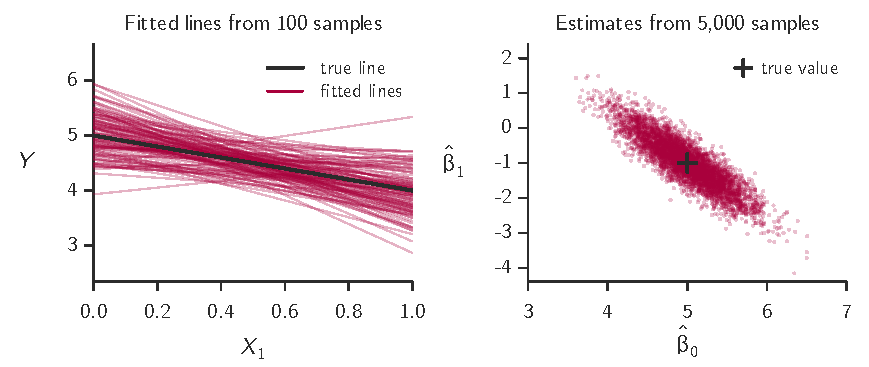
\includegraphics[height=0.61\textheight]{sim_joint_lines.pdf}
\end{figure}
\slidesource{simulation; $X_1$ drawn once from $U(0,1)$ and held fixed across 5{,}000 samples.}
}


\frame{
\frametitle{Marginal Sampling Distribution}
\scriptsize
$Y = \beta_0 + \beta_1 X_1+u$ with $u\sim N(0,\sigma^2_u=4)$ and $\beta_0=5$, $\beta_1=-1$, and $n=100$:
\vspace{-.3cm}
\begin{figure}[ht] \centering
        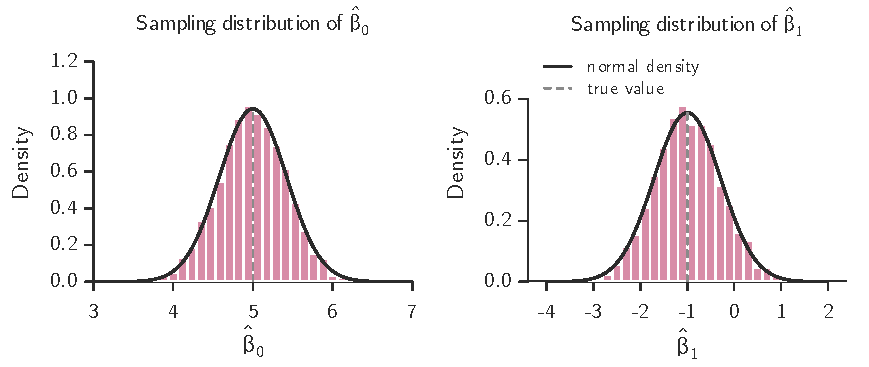
\includegraphics[height=0.61\textheight]{sim_joint_marginals.pdf}
\end{figure}
\slidesource{simulation; $X_1$ drawn once from $U(0,1)$ and held fixed across 5{,}000 samples.}

}

\frame{
\frametitle{Joint Sampling Distribution}
\scriptsize
$Y = \beta_0 + \beta_1 X_1+u$ with $u\sim N(0,\sigma^2_u=4)$ and $\beta_0=5$, $\beta_1=-1$, and $n=100$:
\vspace{-.3cm}
\begin{figure}[ht] \centering
        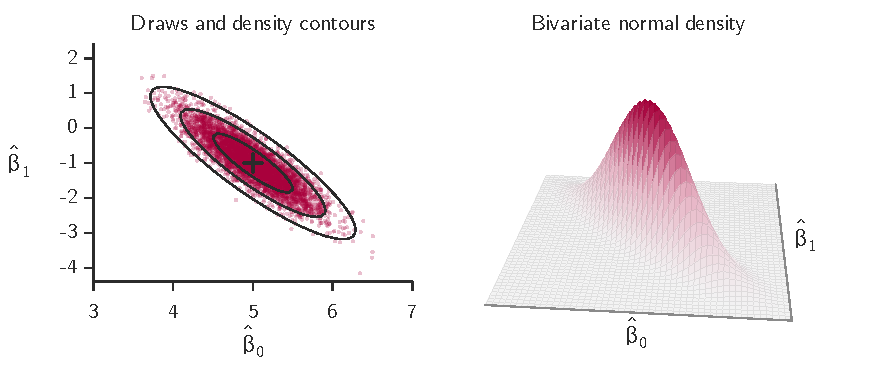
\includegraphics[height=0.61\textheight]{sim_joint_density.pdf}
\end{figure}The true \alert{variance-covariance matrix} of the estimators, $\sigma^2_u(\X'\X)^{-1}$, is:
\begin{tabular}{c|cc}
           &    $\widehat{\beta}_0$ &    $\widehat{\beta}_1$  \\
\hline
   $\widehat{\beta}_0$ & $.18$ & $-.27$        \\
   $\widehat{\beta}_1$ & $-.27$ & $.52$                  \\
\end{tabular}
\slidesource{simulation; $X_1$ drawn once from $U(0,1)$ and held fixed across 5{,}000 samples. The draws give variances $.18$ and $.50$ and covariance $-.26$.}
}

%\frame{
%\frametitle{Variance-Covariance Matrix}
%
%The \alert{variance-covariance matrix} of the OLS estimators is given by:
%\begin{table}
%\begin{center}
%\begin{tabular}{c|cc}
%           &    $\widehat{\beta}_0$ &    $\widehat{\beta}_1$  \\
%\hline
%   $\widehat{\beta}_0$ & $.08$ & $-.11$          \\
%   $\widehat{\beta}_1$ & $-.11$ & $.24$                  \\
%\end{tabular}
%\end{center}
%\end{table}
%
%}



\begin{frame}[fragile]
\frametitle{Example: Is the 1-2-3 Coding of Education OK?}
\footnotesize

\begin{Verbatim}[fontsize=\footnotesize, frame=single, label=R Code, commandchars=\\\{\}]
> fit.dum <- lm(vote1 ~ fem + age + S + PS, data = d)
> V <- vcov(fit.dum)
> V
              (Intercept)           fem           age             \alert{S}
(Intercept)  1.903067e-03 -3.393292e-04 -3.121865e-05 -6.786308e-04
fem         -3.393292e-04  5.581411e-04  1.019330e-06  4.685980e-05
age         -3.121865e-05  1.019330e-06  6.969858e-07  6.908035e-06
\alert{S}           -6.786308e-04  4.685980e-05  6.908035e-06  \alert{7.613989e-04}
\alert{PS}          -6.961468e-04  7.344137e-05  6.987371e-06  \alert{4.232502e-04}
                       \alert{PS}
(Intercept) -6.961468e-04
fem          7.344137e-05
age          6.987371e-06
\alert{S}            \alert{4.232502e-04}
\alert{PS}           \alert{1.111396e-03}
\end{Verbatim}
\end{frame}

\begin{frame}[fragile]
\frametitle{Example: Is the 1-2-3 Coding of Education OK?}
\footnotesize
 We can then compute the test statistic for the hypothesis of interest:


\vspace{-.25\baselineskip}
\begin{eqnarray*}
& & t = \frac{\widehat{\beta}_{PS}-2\widehat{\beta}_{S}}{\widehat{SE}(\widehat{\beta}_{PS}-2\widehat{\beta}_{S})} \quad \quad \text{where} \\\bigskip
& & \widehat{SE}(\widehat{\beta}_{PS}-2\widehat{\beta}_{S})=\sqrt{\widehat{V}(\widehat{\beta}_{PS}) + 4\widehat{V}(\widehat{\beta}_{S}) - 4\widehat{\cov}[\widehat{\beta}_{S},\widehat{\beta}_{PS}]}
\end{eqnarray*}
\vspace{-.5\baselineskip}


\begin{Verbatim}[fontsize=\footnotesize, frame=single, label=R Code, commandchars=\\\{\}]
> se <- sqrt(V["PS","PS"] + 4*V["S","S"] - 4*V["S","PS"])
> se
[1] 0.0496386
>
> tstat <- (coef(fit.dum)["PS"] - 2*coef(fit.dum)["S"])/se
> tstat
      PS
1.046326
\end{Verbatim}

Dropping the covariance term would inflate the SE from 0.0496 to 0.0645.
Plugging in we get $t \simeq 1.05$. So what do we conclude?

\pause
\medskip

We cannot reject the null ($p = 0.30$). The data are consistent with the 1-2-3 coding, under which the Yes-vote gap between post-secondary and primary is twice the gap between secondary and primary.

\end{frame}


\section{Testing Joint Significance}


\frame{
\frametitle{$F$ Test for Joint Significance of Coefficients}
\footnotesize
\begin{itemize}

\item In research we often want to test a \alert{joint hypothesis} which involves \alert{multiple linear restrictions} (e.g. $\beta_1=\beta_2=\beta_3=0$)
\item Suppose our regression model is:
\[Vote=\beta_0+ \gamma_1 FEMALE + \beta_1 EDUCATION +\]\[ \gamma_2
(FEMALE\cdot EDUCATION) + \beta_2 AGE + \gamma_3 (FEMALE\cdot AGE)+u\]
and we want to test
$$H_0: \ \gamma_1=\gamma_2=\gamma_3=0.$$
\pause
\vspace{-\baselineskip}
\item Substantively, what question are we asking? \\
\smallskip
\pause
$\rightarrow$ Do females and males vote systematically differently from each other? \\
(Under the null, there is no difference
in either the intercept or slopes between females and males).
\pause
\item This is an example of a joint hypothesis test involving \alert{three restrictions}:
$\gamma_1=0$, $\gamma_2=0$, and $\gamma_3=0$.
\item If the three estimates are jointly close to zero, relative to their sampling variability, we fail to reject the null of no gender difference.
\item \alert{$F$ tests} allow us to test \alert{joint hypotheses}
\end{itemize}
}





\frame{
\frametitle{The $\chi^2$ Distribution}
\footnotesize

\begin{itemize}
  \item To test more than one hypothesis jointly we need some additional probability distributions.
  \item Suppose $Z_1, ..., Z_n$ are $n$ i.i.d. random variables following $\cN(0,1)$.
  \item Then, the \alert{sum of their squares}, $X = \sum_{i=1}^n Z_i^2$, is distributed
according to the \pause \alert{$\chi^2$ distribution} with $n$ degrees of freedom,
$X \sim \chi_n^2$.
\end{itemize}

\pause
\vspace{-.75\baselineskip}
\begin{center}
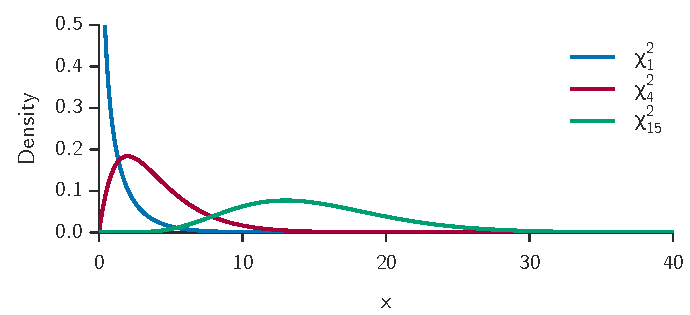
\includegraphics[height=.6\textheight]{chisq_densities}
\end{center}
\vspace{-1.5\baselineskip}
Properties: $X > 0$, $E[X] = n$ and $V[X] = 2n$. In \texttt{R}: \texttt{dchisq()}, \texttt{pchisq()}, \texttt{rchisq()}
}

\frame{
\frametitle{The $F$ distribution}
\footnotesize
The \alert{F distribution} arises as a ratio of two independent
chi-squared distributed random variables:
\[
    F \ = \ \frac{X_1/df_1}{X_2/df_2} \ \sim \ \mathcal{F}_{df_1,df_2}
\]
where $X_1\sim \chi^2_{df_1}$, $X_2\sim \chi^2_{df_2}$, and $X_1 \indep X_2$.

\pause
\bigskip

$df_1$ and $df_2$ are called the \alert{numerator degrees of freedom} and the \alert{denominator degrees of freedom}. 

In \texttt{R}: \texttt{df()}, \texttt{pf()}, \texttt{rf()}
\vspace{-.5\baselineskip}
\begin{figure}[ht] \centering
  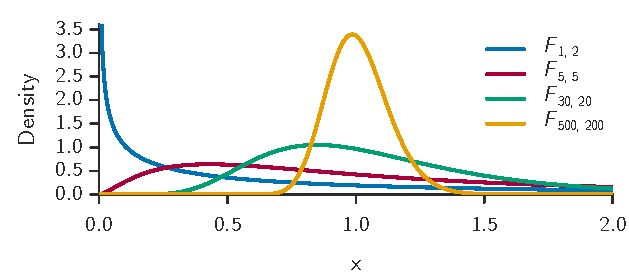
\includegraphics[height=.46\textheight]{f_densities.pdf}
\end{figure}


%
%
%Example: Suppose we have two sample means $\bar{y}_1$ and $\bar{y}_2$ from
%independent normal samples with $n_1$ and $n_2$ observations. Then the ratio of the
%variances of the sample means:
%\[
%F_0=\hat{\sigma}_{\bar{y}_1}/\hat{\sigma}_{\bar{y}_2}
%\]
%is $F_0$ distributed.% Why and what are the $df$ for $F_0$?
%%Recall that the (scaled) sample variance is $\sim \chi^2{n-1}$
}





\frame{
\frametitle{$F$ Test against $H_0: \ \gamma_1=\gamma_2=\gamma_3=0.$}
\footnotesize
The \alert{$F$ statistic} can be calculated by the following procedure:
\begin{enumerate}
\item Fit the \alert{unrestricted model (ur)} which {\it does not} impose $H_0$:
\[Vote=\beta_0+ \gamma_1 FEM + \beta_1 EDUC + \gamma_2 (FEM*EDUC) +
\beta_2 AGE + \gamma_3 (FEM*AGE)+u\]
\pause
\vspace{-\baselineskip}
\item Fit the \alert{restricted model (r)} which {\it does} impose $H_0$:
\[Vote=\beta_0+ \beta_1 EDUC + \beta_2 AGE + u\]
\pause
\vspace{-\baselineskip}

\item From the two results, compute the \alert{$F$ statistic:}
  $$F_0=\frac{(SSR_r-SSR_{ur})/q}{SSR_{ur}/(n-k-1)}$$
where \alert{SSR}$=$sum of squared residuals, \alert{q}$=$number of restrictions, \alert{$k$}=number of predictors in the unrestricted model, and \alert{$n$}= \# of observations. \\ \pause
\medskip
Note that $F_0$ measures relative increase in (minimized) SSR when going from UR to R.
\end{enumerate}

\pause
\medskip

The $F$ statistics have the following sampling distributions:
\begin{itemize}
  \item If $H_0$ is true and Assumptions I--VI hold, $F_0 \sim \mathcal{F}_{q, n-k-1}$ regardless of the sample size.
  \item If $H_0$ is true and Assumptions I--V hold, $q\,F_0 \stackrel{a.}{\sim} \chi^2_{q}$ as $n \to \infty$
  (see next section).
\end{itemize}
}

\begin{frame}[fragile]
\frametitle{Unrestricted Model (UR)}

\begin{Verbatim}[fontsize=\scriptsize, frame=single, label=R Code, commandchars=\\\{\}]
> fit.UR <- lm(vote1 ~ fem + educ + age + fem:age + fem:educ, data = Chile)
> summary(fit.UR)
~~~~~
Coefficients:
             Estimate Std. Error t value Pr(>|t|)
(Intercept)  0.358278   0.068998   5.193 2.32e-07 ***
fem          0.421666   0.100858   4.181 3.05e-05 ***
educ        -0.071545   0.022437  -3.189  0.00146 **
age          0.005198   0.001094   4.752 2.19e-06 ***
fem:age     -0.004228   0.001657  -2.551  0.01082 *
fem:educ    -0.073680   0.032931  -2.237  0.02539 *
---
Signif. codes:  0 `***' 0.001 `**' 0.01 `*' 0.05 `.' 0.1 ` ' 1

Residual standard error: 0.4835 on 1697 degrees of freedom
Multiple R-squared: 0.06785,	Adjusted R-squared: 0.06511
F-statistic: 24.71 on 5 and 1697 DF,  p-value: < 2.2e-16
\end{Verbatim}

\end{frame}

\begin{frame}[fragile]
\frametitle{Restricted Model (R)}

\begin{Verbatim}[fontsize=\footnotesize, frame=single, label=R Code, commandchars=\\\{\}]
> fit.R <- lm(vote1 ~ educ + age, data = Chile)
> summary(fit.R)
Coefficients:
              Estimate Std. Error t value Pr(>|t|)
(Intercept)  0.5773293  0.0505810  11.414  < 2e-16 ***
educ        -0.1138543  0.0165133  -6.895 7.58e-12 ***
age          0.0031356  0.0008293   3.781 0.000162 ***
---

Residual standard error: 0.4886 on 1700 degrees of freedom
Multiple R-squared:  0.04662,	Adjusted R-squared:  0.0455
F-statistic: 41.56 on 2 and 1700 DF,  p-value: < 2.2e-16
\end{Verbatim}

\end{frame}


\begin{frame}[fragile]
\frametitle{$F$ Test in R}
\begin{Verbatim}[fontsize=\footnotesize, frame=single, label=R Code, commandchars=\\\{\}]
> SSR.UR <- sum(resid(fit.UR)^2)  # = 396.7
> SSR.R <- sum(resid(fit.R)^2)    # = 405.8

> DFdenom <- df.residual(fit.UR)  # = 1697
> DFnum <- 3

> F <- ((SSR.R - SSR.UR)/DFnum) / (SSR.UR/DFdenom)
> F
[1] 12.88682

> qf(0.99, DFnum, DFdenom)
[1] 3.793171
\end{Verbatim}
Given above, what do we conclude? \\ \pause
$F_0 \approx 12.89$ is greater than the \alert{critical value} for a $.01$ level test. So we
{\it reject} the null hypothesis.

\end{frame}

\frame{
\frametitle{Null Distribution, Critical Value, and Test Statistic}
\small
Large values of $F$ mean that imposing $H_0$ raised the SSR a lot, so we reject only in the right tail of $\mathcal{F}_{q,n-k-1}$ (in large samples, compare $qF_0$ with $\chi^2_q$).
\begin{figure}[ht] \centering
        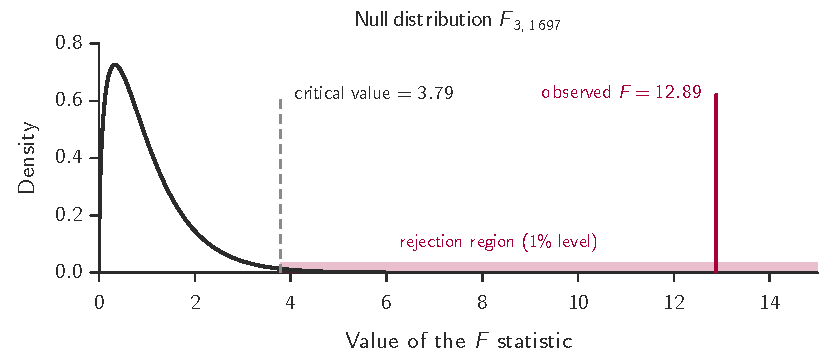
\includegraphics[height=0.69\textheight]{f_null_chile.pdf}
\end{figure}

}


\frame[t]{
\frametitle{$F$ Test Example 1: The ``Omnibus Test''}
\textbf{Worksheet Q2}\\ \medskip\small
Consider the multiple regression model
\[
Y = \beta_0 + \beta_1 X_1 + \beta_2 X_2 + \cdots + \beta_k X_k + u,
\]
and suppose we wish to test the joint null hypothesis
\[
H_0:\ \beta_1=\beta_2=\cdots=\beta_k=0
\quad\text{versus}\quad
H_1:\ \text{at least one }\beta_j\neq 0.
\]

\begin{enumerate}
\item Explain in words what this hypothesis is asking about the explanatory power of the regressors.
\item Describe step-by-step how to conduct the $F$ test for this hypothesis, including:
  \begin{enumerate}
    \item the unrestricted and restricted models,  
    \item how to compute the $F$ statistic from the two sum of squared residuals, and  
    \item how to determine whether to reject $H_0$ at significance level $\alpha$.
  \end{enumerate}
\item Interpret the meaning of rejecting versus not rejecting $H_0$ in terms of the overall explanatory power of $X_1,\ldots,X_k$.
\end{enumerate}

}

% \frame[t]{
% \frametitle{$F$ Test Example I: The Omnibus Test}
% \small
% The $F$ test can be used to test various joint hypotheses which involve multiple linear restrictions.
% Consider the regression model:
% \[Y=\beta_0+\beta_1 X_1 + \beta_2 X_2 + \beta_3 X_3 +...+ \beta_k X_k + u\]
% We may want to test:
%  $$ H_0: \beta_1=\beta_2=...=\beta_k=0$$
% \pause
% \begin{itemize}
%   \item What question are we asking? \\ \medskip \pause
%   $\rightarrow$ Does any of the $X$ variables help to predict $Y$? \medskip
%   \item This is called the \alert{omnibus test} and is routinely reported by statistical software.
% \end{itemize}
% }

\begin{frame}[fragile]
\frametitle{Omnibus Test in R}

\begin{Verbatim}[fontsize=\footnotesize, frame=single, label=R Code, commandchars=\\\{\}]
> summary(fit.UR)
~~~~~
Coefficients:
             Estimate Std. Error t value Pr(>|t|)
(Intercept)  0.358278   0.068998   5.193 2.32e-07 ***
fem          0.421666   0.100858   4.181 3.05e-05 ***
educ        -0.071545   0.022437  -3.189  0.00146 **
age          0.005198   0.001094   4.752 2.19e-06 ***
fem:age     -0.004228   0.001657  -2.551  0.01082 *
fem:educ    -0.073680   0.032931  -2.237  0.02539 *
---

Residual standard error: 0.4835 on 1697 degrees of freedom
Multiple R-squared: 0.06785,	Adjusted R-squared: 0.06511
\alert{F-statistic: 24.71 on 5 and 1697 DF,  p-value: < 2.2e-16}
\end{Verbatim}
\end{frame}



\frame[t]{
\frametitle{$F$ Test Example 2: Equality of Coefficients}
\textbf{Worksheet Q3}\\ \medskip\small
Consider the multiple regression model
\[
Y = \beta_0 + \beta_1 X_1 + \beta_2 X_2 + \beta_3 X_3 + \cdots + \beta_k X_k + u,
\]
and suppose we want to test whether the first three regressors have the same effect:
\[
H_0:\ \beta_1=\beta_2=\beta_3 \quad \text{versus} \quad H_1:\ \text{at least one differs.}
\]

\begin{enumerate}
\item Describe the step-by-step $F$ test procedure, including:
  \begin{enumerate}
    \item how to construct the restricted model implied by $H_0$,
    \item how to compute the $F$ statistic using the two sums of squared residuals, and
    \item the reference distribution used for inference.
  \end{enumerate}
\item Provide an intuitive interpretation of what rejecting or failing to reject $H_0$ implies about the coefficients on $X_1$, $X_2$, and $X_3$ in the regression for $Y$.
\end{enumerate}
}

% \frame{
% \frametitle{$F$ Test Examples II}
% \small
% The $F$ test can be used to test various joint hypotheses which involve multiple linear restrictions.
% Consider the regression model:
% \[Y=\beta_0+\beta_1 X_1 + \beta_2 X_2 + \beta_3 X_3 +...+ \beta_k X_k + u\]
% Next, let's consider:
%  $$ H_0: \beta_1 = \beta_2 = \beta_3 $$
% \pause
% \vspace{-\baselineskip}
% \begin{itemize}
%   \item What question are we asking?  \\ \smallskip \pause
%     $\rightarrow$ Are the effects of $X_1$, $X_2$ and $X_3$ different from each other?
%     \medskip \pause
%   \item How many restrictions? \\ \smallskip \pause
%     $\rightarrow$ Two ($\beta_1-\beta_2=0$ and $\beta_2 - \beta_3 =0$)
%     \medskip \pause
%   \item How do we fit the restricted model? \\ \smallskip \pause
%     $\rightarrow$ The null hypothesis implies that the model can be written as:
% \[Y = \beta_0 + \beta_1(X_1 + X_2 + X_3) + ... + \beta_k X_k + u \]
%     So we create a new variable $X^\ast = X_1 + X_2 + X_3$ and fit: $Y = \beta_0 + \beta_1 X^\ast + ... + \beta_k X_k + u$

% \end{itemize}
% }

\begin{frame}[fragile]
\frametitle{Testing Equality of Coefficients in R}

\begin{Verbatim}[fontsize=\footnotesize, frame=single, label=R Code, commandchars=\\\{\}]
> fit.dum <- lm(vote1 ~ fem + age + S + PS, data = d)
> summary(fit.dum)
~~~~~
Coefficients:
              Estimate Std. Error t value Pr(>|t|)
(Intercept)  0.4005593  0.0436242   9.182  < 2e-16 ***
fem          0.1280018  0.0236250   5.418 6.89e-08 ***
age          0.0032133  0.0008349   3.849 0.000123 ***
\alert{S           -0.1283286  0.0275935  -4.651 3.56e-06 ***}
\alert{PS          -0.2047191  0.0333376  -6.141 1.02e-09 ***}
---
Signif. codes:  0 `***' 0.001 `**' 0.01 `*' 0.05 `.' 0.1 ` ' 1

Residual standard error: 0.4845 on 1698 degrees of freedom
Multiple R-squared:  0.06353,	Adjusted R-squared:  0.06132
F-statistic:  28.8 on 4 and 1698 DF,  p-value: < 2.2e-16
\end{Verbatim}
Are the coefficients on $S$ and $PS$ statistically significantly different?\\
{\footnotesize Under $H_0: \beta_S=\beta_{PS}$, secondary and post-secondary voters differ from primary-school voters by the same amount.}
\end{frame}


\begin{frame}[fragile]
\frametitle{Testing Equality of Coefficients in R}

\begin{Verbatim}[fontsize=\footnotesize, frame=single, label=R Code, commandchars=\\\{\}]
> d$Xstar <- d$S + d$PS
> fit.R2 <- lm(vote1 ~ fem + age + Xstar, data = d)

> SSR.UR2 <- sum(resid(fit.dum)^2)
> SSR.R2 <- sum(resid(fit.R2)^2)

> DFdenom <- df.residual(fit.dum)

> F <- ((SSR.R2 - SSR.UR2)/1) / (SSR.UR2/DFdenom)
> F
[1] 5.685995

> pf(F, 1, DFdenom, lower.tail = FALSE)
[1] 0.01721005
\end{Verbatim}
So, what do we conclude? \\ \pause
We reject the null that the two coefficients are the same at the .05 level, with
a p-value of $0.017$.

\end{frame}


\frame{
\frametitle{$t$ Test vs. $F$ Test}
\small
Consider the hypothesis test of
$$ H_0: \ \beta_1 = \beta_2 \quad \text{vs.} \quad H_1: \ \beta_1 \neq \beta_2 $$
What ways have we learned to conduct this test?
\pause
\begin{itemize}
  \item Option 1: Compute $T = (\hat\beta_1 - \hat\beta_2)/\widehat{SE}(\hat\beta_1 - \hat\beta_2)$ and
    do the \alert{t test}. \pause
  \item Option 2: Create $X^\ast = X_1 + X_2$, fit the restricted model, compute
    $F = (SSR_{R} - SSR_{UR})\big/(SSR_{UR}/(n-k-1))$ and do the \alert{$F$ test}.
\end{itemize}
\pause
\medskip
It turns out the $F$ test and the two-sided $t$ test give \alert{identical} results. This is because $F = T^2$ in every sample, and
$$ X \ \sim \ t_{n-k-1} \quad \Longrightarrow \quad X^2 \ \sim \ \mathcal{F}_{1,n-k-1}$$
{\footnotesize (The arrow does not reverse: $|X|^2 \sim \mathcal{F}_{1,n-k-1}$ as well, but $|X|$ is never negative, so it is not $t$ distributed.)}
\pause
\begin{itemize}
  \item So, for one linear restriction, the $F$ test and the two-sided $t$ test give the same answer.
  \item Usually, the $t$ test is used for single hypotheses and the $F$ test is used for joint
    hypotheses.
\end{itemize}

}

\frame{
\frametitle{Some More Notes on $F$ Tests}
\small
\begin{itemize}
  \item When both models have the same outcome variable and observations, the F-value can also be calculated from $R^2$:
    $$ F \ = \ \frac{(R_{UR}^2-R_{R}^2)/q}{(1-R_{UR}^2)/(n-k-1)}$$
\pause
  \item $F$ tests only work for testing \alert{nested} models, i.e. the restricted model
    must be a special case of the unrestricted model. \\ \medskip
    For example $F$ tests cannot be used to test
    $$ Y \ = \ \beta_0 + \beta_1 X_1 \invisible{+ \beta_2 X_2} + \beta_3 X_3 + u $$
    against
    $$ Y \ = \ \beta_0 + \beta_1 X_1 + \beta_2 X_2 + \invisible{\beta_3 X_3} + u $$
\end{itemize}
}

\frame{
\frametitle{Some More Notes on $F$ Tests}
\small
\begin{itemize}
  \item Joint significance does not necessarily imply the significance of
    individual coefficients, or vice versa:
\end{itemize}
{\centering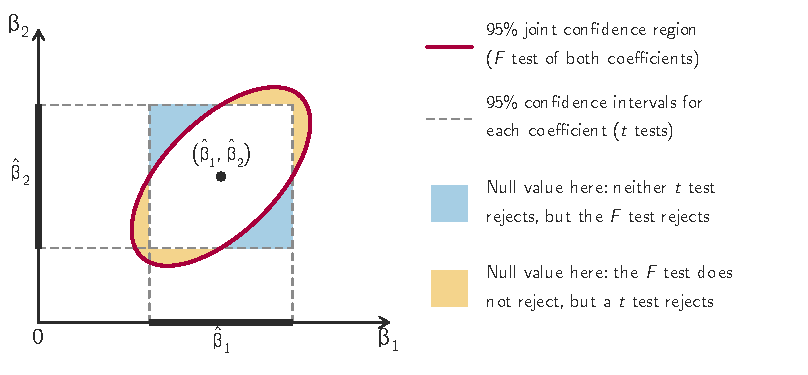
\includegraphics[height=0.70\textheight]{t_vs_f_region.pdf}\par}
\slidesource{Hayashi, \emph{Econometrics} (2000), Fig.~1.5 (``$t$- versus $F$-tests''), redrawn}

}

\begin{frame}[fragile]
\frametitle{When $t$ and $F$ Disagree: Age and Age$^2$ in Chile}

\begin{Verbatim}[fontsize=\footnotesize, frame=single, label=R Code, commandchars=\\\{\}]
> fit.sq <- lm(vote1 ~ fem + educ + age + I(age^2), data = d)
> summary(fit.sq)
Coefficients:
              Estimate Std. Error t value Pr(>|t|)
(Intercept)  4.438e-01  9.811e-02   4.523 6.50e-06 ***
fem          1.274e-01  2.370e-02   5.375 8.74e-08 ***
educ        -1.057e-01  1.648e-02  -6.412 1.86e-10 ***
\alert{age          6.105e-03  4.814e-03   1.268    0.205}
\alert{I(age^2)    -3.301e-05  5.699e-05  -0.579    0.563}

> fit.noage <- lm(vote1 ~ fem + educ, data = d)
> anova(fit.noage, fit.sq)
  Res.Df    RSS Df Sum of Sq      F    Pr(>F)
1   1700 402.73
2   1698 398.75  2    3.9807 8.4754 \alert{0.0002175} ***
\end{Verbatim}
\small
\pause
Neither age term is significant on its own ($p = 0.20$ and $0.56$), yet together they are ($F = 8.48$, $p = 0.0002$).
\pause
Age and age$^2$ move together (correlation 0.99), so the data cannot tell which of the two terms carries the age pattern, and each SE is large. Dropping both terms raises the SSR from 398.75 to 402.73, more than chance would explain. In the figure on the last slide, our null value $(0,0)$ lies in a blue area, inside the box but outside the ellipse.
\end{frame}

\section{Testing Linear Hypotheses: The General Case}

\frame{
\frametitle{Limitation of the F Formula}
Consider the following null hypothesis:
$$ H_0: \ \beta_1 = \beta_2 = \beta_3 = 3 $$
or
$$ H_0: \ \beta_1 = 2\beta_2 = 0.5\beta_3 + 1 $$
Can we test them using the $F$ test? \\ \pause
To compute the F value, we need to fit the restricted model. How? \\ \pause
\medskip
\begin{itemize}
  \item Some restrictions are difficult to impose when fitting the model.
  \item Even when we can, the procedure will be ad hoc and require some creativity. \pause
  \item Is there a general solution?
\end{itemize}

}


\frame{
\frametitle{General Procedure for Testing Linear Hypotheses}
\small
\begin{itemize}
  \item Notice that any set of $q$ linearly independent linear restrictions can be written as
    $$ \mb{R} \b \ = \ \mb{r} $$
    where
    \begin{itemize}
      \addtolength{\itemsep}{.25\baselineskip}
      \item $\mb{R}$ is a $q \times (k + 1)$ matrix of prespecified coefficients on $\b$ (\alert{hypothesis matrix}); $\mb{R}$ has rank $q$
      \item $\b = [\beta_0 \ \beta_1 \ \cdots \ \beta_k]'$
      \item $\mb{r}$ is a $q \times 1$ vector of prespecified constants
    \end{itemize}
% \bigskip
% \pause
%   \item Examples: \pause
%     {\scriptsize
%     $$\hspace{-20pt} \beta_1 = \beta_2 = \beta_3 = 3 \ \Leftrightarrow \
%     \l[\begin{array}{c} \beta_1 \\ \beta_2 \\ \beta_3 \end{array}\r] =
%     \l[\begin{array}{c} 3 \\ 3 \\ 3 \end{array}\r]
%     \ \Leftrightarrow \
%     \l[\begin{array}{cccc} 0 & 1 & 0 & 0 \\ 0 & 0 & 1 & 0 \\ 0 & 0 & 0 & 1 \end{array} \r] \cdot
%     \l[\begin{array}{c} \beta_0 \\ \beta_1 \\ \beta_2 \\ \beta_3 \end{array} \r] =
%     \l[\begin{array}{c} 3 \\ 3 \\ 3 \end{array}\r] $$ \pause
%     $$\hspace{-25pt} \beta_1 = 2\beta_2 = 0.5\beta_3 + 1 \ \Leftrightarrow \
%     \l[\begin{array}{c} \beta_1 - 2\beta_2 \\ \beta_1 - 0.5\beta_3 \end{array}\r] =
%     \l[\begin{array}{c} 0 \\ 1 \end{array}\r]
%     \ \Leftrightarrow \
%     \l[\begin{array}{cccc} 0 & 1 & -2 & 0 \\ 0 & 1 & 0 & -0.5 \end{array} \r] \cdot
%     \l[\begin{array}{c} \beta_0 \\ \beta_1 \\ \beta_2 \\ \beta_3 \end{array} \r] =
%     \l[\begin{array}{c} 0 \\ 1 \end{array}\r] $$
%     }
\end{itemize}
}

\frame{
\frametitle{General Procedure for Testing Linear Hypotheses}
\textbf{Worksheet Q4} Consider the linear regression model
\[
Y = \beta_0 + \beta_1 X_1 + \beta_2 X_2 + \beta_3 X_3 + u,
\]
with coefficient vector $\b = [\beta_0\ \beta_1\ \beta_2\ \beta_3]'$. We wish to test linear hypotheses of the form $R\b=r$. Construct the corresponding $R$ and $r$ in the following two scenarios.
\begin{enumerate}
\item Test the hypothesis that all three slope coefficients equal 3:
\[
H_0:\ \beta_1=\beta_2=\beta_3=3.
\]
Write this null hypothesis in matrix form $R\b=r$ by explicitly constructing $R$ and $r$.

\item Test the joint hypothesis
\[
H_0:\ \beta_1 = 2\beta_2 = 0.5\beta_3 + 1.
\]
\end{enumerate}
}


\frame{
\frametitle{Wald Statistic}
\small
\begin{itemize}
  \item Let's consider testing $H_0: \mb{R}\b = \mb{r}$, a set of $q$ linearly independent linear restrictions.
\pause
  \item If $H_0$ is true, $\mb{R}\hat\b - \mb{r}$ should be zero except for sampling variability.
\pause
  \item To formally evaluate the statistical significance of the deviation from zero,
    we must transform $\mb{R}\hat\b - \mb{r}$ to a \alert{statistic} that can be compared to
    a \alert{reference distribution}.
\pause
  \item It turns out that the following \alert{Wald statistic} can be used:
    $$ W \ = \ \alert<6>{\l(\mb{R}\hat\b - \mb{r}\r)'}
    \cdot \l[ \alert<7>{\hat\sigma^2\mb{R}(\XX)^{-1}\mb{R}'} \r]^{-1}
    \cdot \alert<6>{\l(\mb{R}\hat\b - \mb{r}\r)} $$
\pause
\vspace{-\baselineskip}
  \item Looks complicated? Let's figure out why this makes sense: \pause
    \begin{itemize}
      \addtolength{\itemsep}{.25\baselineskip}
      \item The first and last components are the deviations $\mb{R}\hat\b - \mb{r}$; on their own they would give a sum of squares. \pause
      \item The middle component is the \alert{inverse} of the estimated variance matrix of $\mb{R}\hat\b - \mb{r}$. It puts each deviation on a standard scale and removes their correlation, so that under $H_0$ the statistic is roughly a sum of $q$ squared standard normals. \pause
    \end{itemize}

  \item We know $\hat\b$ is approximately normal $\Rightarrow$ $\mb{R}\hat\b - \mb{r}$
    should also be normal \\
    $\Longrightarrow$ $W$ should therefore be ... \pause \alert{$\chi^2$} distributed!
\end{itemize}
}

\frame{
\frametitle{Sampling Distribution of the Wald Statistic}

\small

\begin{theorem}[Large-Sample Distribution of the Wald Statistic]
\footnotesize
If $H_0$ is true, then under Assumptions I--V, as $n \to \infty$ the distribution of the Wald statistic
approaches the chi square distribution with $q$ degrees of freedom:
\vspace{-.25\baselineskip}
$$
W \ \stackrel{d}{\to} \ \chi^2_q
\quad \text{as} \quad n \to \infty
$$
\end{theorem}
\begin{theorem}[Small-Sample Distribution of the Wald Statistic]
\footnotesize
If $H_0$ is true, then under Assumptions I--VI, for any sample size $n$ the Wald statistic divided by $q$
has the F distribution with $(q, n - k - 1)$ degrees of freedom:
\vspace{-.25\baselineskip}
$$
W/q \ \sim \ \mathcal{F}_{q, n-k-1}
$$
\end{theorem}
\begin{itemize}
  \item $q\mathcal{F}_{q,n-k-1}\stackrel{d}{\to} \chi^2_q$ as $n\to\infty$,
    so the difference disappears when $n$ large.\\
\tiny{ \texttt{> pf(3.1, 2, 500, lower.tail=FALSE)
[1] 0.04591619\\\medskip
> pchisq(2*3.1, 2, lower.tail=FALSE)
[1] 0.0450492\\
> pf(3.1, 2, 50000, lower.tail=FALSE)
[1] 0.04505786
 }
 }    \small
 % \item In practice people often just use $\mathcal{F}_{q,n-k-1}$ to be on the conservative side.
%  \item It turns out that $W/q$ is \alert{numerically equal} to the $F$ value. But $W$ does not
 %   require the estimation of the restricted model.
\end{itemize}



}


\begin{frame}[fragile]
\frametitle{Testing General Linear Hypotheses in R}
\small
In R, the {\tt linearHypothesis()} function
in the {\tt car} package does the Wald test for general linear hypotheses.

\medskip

\begin{Verbatim}[fontsize=\scriptsize, frame=single, label=R Code, commandchars=\\\{\}]
> fit.dum <- lm(vote1 ~ fem + age + S + PS, data = d)
> R <- matrix(c(0, 0, 0, -2, 1), nrow = 1)
> r <- 0
> linearHypothesis(fit.dum, R, r)
Linear hypothesis test:
- 2 S  + PS = 0

Model 1: restricted model
Model 2: vote1 ~ fem + age + S + PS

  Res.Df    RSS Df Sum of Sq      F Pr(>F)
1   1699 398.83
2   1698 398.57  1   0.25698 1.0948 0.2956
\end{Verbatim}
\pause
This is the test of the 1-2-3 coding again, and $F = 1.09 = 1.046^2 = t^2$. Here the restricted model is also easy to fit. Under $H_0$, $\beta_S S + \beta_{PS} PS = \beta_S(S + 2PS) = \beta_S(educ - 1)$, so the restricted model is our first model, \mbox{\texttt{lm(vote1 \textasciitilde{} fem + educ + age)}}.
\end{frame}

%\frame{
%\frametitle{Problem of Multiple Testing}
%\begin{itemize}
%\item The multiple testing (or ``multiple comparison'') problem occurs when one considers a set o$F$ statistical tests simultaneously.
%\item Consider $k=1,...,m$ independent hypothesis tests (e.g. control versus various treatment groups). Even if each test is carried out at a low significance level (e.g., $\alpha=0.05$) the \alert{over all type I error rate} grows very fast:\\
%    $\alpha_{overall}=1-(1-\alpha_{k})^m$.
%\item That's right - it grows exponentially. E.g., given test 7 tests at $\alpha=.1$ level the overall type I error is $.52$.
%\item Even if all null hypotheses are true we will
%reject at least one of them with probability $.52$.
%\item Same for confidence intervals: probability that all 7 CI cover the true values simultaneously
%over repeated samples is $.52$. So for each coefficient you have a .90 confidence interval, but overall a
%.52 percent confidence interval.
%%\item Several statistical techniques have been developed to ``adjust'' for this inflation of overall type I errors for multiple testing. These techniques generally require a stronger level of evidence to be observed in order for an individual comparison to be deemed ``significant'' so as to compensate for the number of inferences being made.
%\end{itemize}
%
%}
%
%\frame{
%\frametitle{Problem of Multiple Testing}
%\begin{itemize}
%\item Several statistical techniques have been developed to ``adjust'' for this inflation of overall type I errors for multiple testing.
%\item To compensate for the number of tests, these corrections generally require a stronger level of evidence to be observed in order for an individual comparison to be deemed ``significant''
%\item The most prominent adjustments include:
%\begin{itemize}
%  \item Bonferroni: for each individual test use significance level of $alpha_{k,BFer}=\alpha_{k}/m$
%  \item Sidak: for each individual test use significance level of $alpha_{k,Sid}=1 - (1 - \alpha_{k})1 / m$
%  \item Scheffe (for confidence intervals)
%\end{itemize}
%\item Some are implemented with \texttt{test} , \texttt{mtest(option)}
%\item It remains a heated debate.
%\end{itemize}
%
%}



\end{document}
